\documentclass[11pt,a4paper]{globis-book}

\usepackage{graphicx}
\usepackage{caption}
\usepackage{subcaption}
\usepackage[helvetica]{quotchap}
\usepackage{times}
\usepackage{ethfont}
\usepackage[british]{babel}
\usepackage{longtable}
\usepackage{fancyhdr}
\usepackage{shadethm}
\usepackage{makeidx}
\usepackage[a4paper,portrait,twoside,inner=3.25cm,outer=3.5cm,top=3.5cm,bottom=4.0cm]{geometry}
\usepackage{hyperref}
\usepackage{globis}

\renewcommand{\sectfont}{\sffamily\bfseries\Huge}
\setlength{\shadedtextwidth}{\textwidth}
\setlength{\shadeleftshift}{3mm}
\setlength{\shaderightshift}{3mm}
\addtolength{\shadedtextwidth}{-\shadeleftshift}
\addtolength{\shadedtextwidth}{-\shaderightshift}
\setlength{\parindent}{0pt}
\setlength{\parskip}{5pt}

\sloppy

\pagestyle{fancy}
\fancyhf{}
\fancyhead[LE,RO]{\sffamily\bfseries\small\thepage}
\fancyhead[LO]{\sffamily\bfseries\small\leftmark}
    \fancyhead[RE]{\sffamily\bfseries\small\rightmark}
\renewcommand{\headrulewidth}{0.1pt}
\renewcommand{\footrulewidth}{0pt}

\fancypagestyle{plain}{
    \fancyhf{}
    \fancyfoot[C]{\sffamily\bfseries\small\thepage}
    \renewcommand{\headrulewidth}{0pt}
    \renewcommand{\footrulewidth}{0pt}
}

% Please adapt the following fields if necessary!
\hypersetup{
    pdftitle = Distributed Ph Tree, 
    pdfauthor = Bogdan Vancea,
    pdfsubject = Master Thesis,
    hidelinks,
    plainpages = false,
    bookmarksnumbered = true
} 

\raggedbottom

% Please adapt the following fields if necessary!
\title{Cluster-Computing and Parallelisation for the
    Multi-Dimensional PH-Index}
\category{Master Thesis} 
\author{Bogdan Aurel Vancea}
\email{$<$bvancea@student.ethz.ch$>$}
\professor{Prof. Dr. Moira C. Norrie}
\assistant{Tilmann Zaeschke \\Christoph Zimmerli}
\group{Global Information Systems Group}
\institute{Institute of Information Systems}
\department{Department of Computer Science}
\school{ETH Zurich}
\version{}
\date{\today}
\copyrightyear{2014}

\makeindex

\begin{document}

\frontmatter
\maketitlepage
\cleardoublepage
\pdfbookmark{Contents}{toc}

\chapter*{Abstract}

Here comes the abstract.

\tableofcontents

\mainmatter

% Here comes the content

\chapter{Introduction}
\label{ch:intro}

\section{Motivation}
\label{sec:intro-motivation}
Multi-dimensional data is widely used today, for example in domains like database management systems, geographic information systems, computer vision and computational geometry. When all of the dimensions of the data hold numerical values, this data can be viewed as a collection of points in higher dimensional spaces. Due to this nature, multi-dimensional numerical data provides the possibility of posing more complex queries based on the distance between these points in space. For example, in the context of a geo-information system, one could query for all of the points that fall inside a specific rectangle or attempt to find the nearest neighbours of an arbitrary query point.

Several point-based multi-dimensional indexing solution have been developed in the latest years, the most prominent being kD-trees~\cite{Bentley1975} and quadtrees~\cite{FinkelB74}. This type of data structures store the multi-dimensional data such that more complex operations, like range and nearest neighbour queries are executed efficiently. The PH-tree~\cite{Zaschke2014} is a new multi-dimensional data structure based on the quadtree. In addition to providing support for complex queries, the PH-tree is also space-efficient, as its space requirements are sometimes even lower than those of multi-dimensional arrays. 

As technology advances and the world becomes more connected, multi-dimensional data becomes easier to acquire and store. Because of this, it is necessary that multi-dimensional data structures need to store and manage more data than would fit in the main memory of a single machine. However, traditional multi-dimensional indexes like the kD-tree and quad-tree do not cover this use case as they are designed to run on a single machine.

Additionally, in the last few years the processor speed has reached the power wall and processor designers cannot increase the CPU frequency by increasing the number of transistors. Recent advances in processor design have been made by adding more cores per CPU rather than increasing the processing frequency. Therefore, it is important that contemporary data structures be adapted to multi-core architectures by allowing them to support concurrent operations. As with the case of the increase storage requirements, traditional multi-dimensional data structures do not support concurrent write operations.

This thesis attempts to provide a solution to these two issues by extending the PH-tree to run on distributed cluster of machines and modifying it to support concurrent operations.

\section{Objectives}
\label{sec:intro-objectives}
We has highlighted two challenges currently faced by indexing systems: \textit{high storage requirements} and \textit{support for concurrent access}. This work proposes the distributed PH-tree, a version of the PH-tree that can be run on a cluster of machines, making it able to handle data sets that cannot fit in the main memory of a single machine. Moreover, the distributed PH-tree should be able to handle concurrent requests. This applies both to requests sent to different machines that are part of the cluster and concurrent requests sent by different clients to the same machine. 

Specifically, the distributed PH-tree has to fulfill the following requirements:
\begin{description}
    \item[Cluster capability] The system should run across a network of machines, making use of the memory and processing resources on each machine. Furthermore, the system should attempt to balance the number of multi-dimensional entries that each machine is responsible of.
    \item[Cluster concurrency] The system should be able to support concurrent requests to different nodes of the cluster. Each node should be able to process queries related to the entries that it stores locally.
    \item[Node concurrency] Each node should support multi-threaded read and write access to the entries that it stores.
\end{description} 

As the thesis touches on two main subjects, distribution and concurrency, the main challenges encountered are twofold. From the distribution perspective, the challenges are the identification of suitable entry distribution and balancing strategies, devising efficient algorithms for executing queries across multiple cluster nodes, and the efficient management of a very large number of cluster nodes. For the concurrency perspective, the challenges are the identification of a suitable concurrent access strategy that can maximize the number of concurrent write operations.

\section{Thesis outline}
\label{sec:intro-outline}

This chapter gave an overview of the challenges currently faced by multi-dimensional indexing structures and briefly explained how this work seeks to address them. Additionally, this chapter also presented the main objectives of this thesis. The rest of the thesis is structured as follows:

\textbf{Chapter \ref{ch:background}} provides additional information about the PH-tree, its characteristics and supported operations. The second part of this chapter describes relevant previous work done in the areas of distributed multi-dimensional indexes and concurrent data structures.

The design of the distributed PH-tree from the point of view of a distributed system is presented in \textbf{Chapter \ref{ch:distindex}}. This chapter presents the chosen data distribution strategy and touches on the possible alternatives and the consequences of this choice. Additionally, we provide an overview of how the queries spanning multiple nodes are executed by the system.

The addition of the multi-threaded read and write support for the PH-tree is presented in \textbf{Chapter \ref{ch:concurrency}}. Several concurrent access strategies are discussed, in terms of their advantages, disadvantages and consistency guarantees.

\textbf{Chapter \ref{ch:implementation}} describes the implementation-specific decisions that were taken during the development process. This chapter also presents the technologies that were used and justifies the technological choices.

The distributed PH-tree is evaluated in \textbf{Chapter \ref{ch:evaluation}}. The performance characteristics of the implemented distributed systems as well as those of the implemented concurrency strategy are discussed.

\textbf{Chapter \ref{ch:conclusions}} concludes the thesis by presenting the contribution of this work in the context of distributed multi-dimensional indexing systems. We also give an outlook of the potential extensions. 

\chapter{Background}
\label{ch:background}
The first part of this chapter analyses the single-threaded PH-tree, a multi-dimensional data structure and the starting point of this work. It provides an overview of its specific characteristics and describes the supported operations.

The second part of this chapter presents the relevant related work in the area of distributed multi-dimensional index and concurrent data structures. 

\section{The PH-tree}
\label{sec:background-phtree}

The PH-tree~\cite{Zaschke2014} is a novel multi-dimensional indexing structure that focuses on fast retrieval, fast update and highly efficient storage. It combines concepts from PATRICIA-tries, quadtrees and hypercubes to encode the multi-dimensional data using bit prefix sharing. Because of this, the storage requirements can sometimes be lower than those of the storage requirements of an array of objects.

An example PH-tree storing 2-dimensional 4 bit points is shown in \ref{fig:PhTree-example}. The tree illustrated in this figure stores the points: (0, 4), (3, 4) and (3, 6). However, each point is stored as the \textit{bit interleaving} of its values in all dimensions. Therefore, the bit interleaving of point (3, 6), represented in binary as (0011, 1010) is 01001110. By storing the points under the \textit{bit interleaving} form, the PH-tree maps the multi-dimensional points into a 1-dimensional space. The 1-dimensional values will be referred to as \textit{Z-values} as they form the \textit{Z-order space filling curve}. 

\begin{figure}[h]
    \centering 
    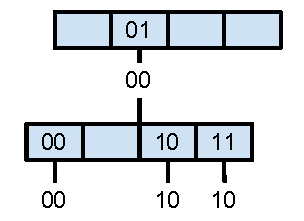
\includegraphics{images/PhTree-example}
    \caption{2 dimensional 4bit PH-tree containing the points: (0000, 1000), (0011, 1000), (0011, 1010).}
    \label{fig:PhTree-example}
\end{figure}

The PH-tree has the following important properties:
\begin{itemize}
    \item \textbf{Z-Ordering}. The multi-dimensional entries are ordered according to the Z-order space filling curve. As a consequence, points which are close in the original multi-dimensional space will usually also be relatively close in the Z-Ordering.
    \item \textbf{Constant maximum height}. The height of the PH-tree is equal the number of bits needed to store each value of the multi-dimensional space. Therefore, when the values in each dimension are represented in 64 bits, as long or doubles, the maximum height of the PH-tree is 64. This property is important as \textit{the maximum height of the PH-tree is independent of the number of points it stores}.
    \item \textbf{Balancing is not needed}. The PH-tree does not perform balancing operation after write operation have occurred. While this fact could lead to un-balanced trees, it is usually not a problem in practice, as the height of tree is limited by a constant factor.
\end{itemize}

The PH-tree is similar to a HashMap, as it stores entries consisting of key-value pairs. In this case however, the key is a multi-dimensional data point, while the value can be an arbitrary object. The following operations are supported:
\begin{itemize}
    \item \textbf{Point operations} operate on single multi-dimensional points. The possible queries are \textit{get()}, \textit{put()}, \textit{delete()} and \textit{updateKey()}. The \textit{get()} query retrieves the value associated with a multi-dimensional key, and the \textit{delete()} operation removes the value associated with a multi-dimensional key. The \textit{put()} operation adds new key-value to the index. Finally, the \textit{updateKey()} operations updates the key associated with an existing key-value entry.
    \item \textbf{Range queries} select all of the data points that fall inside a multi-dimensional hyper-rectangle. This rectangle is defined by a \textit{lower left} and a \textit{upper right} point. 
    \item \textbf{Nearest neighbour queries} select the closest k points in the index to an arbitrary query point. 
\end{itemize}

Currently, the amount of entries the PH-tree can store limited by the memory available on a single host. A distributed version of the PH-tree would be able to store a much larger amount of entries and would be able to make use of clusters of computing nodes. Specifically, the distributed version would be well suited for running in cloud environments, where users can easily add more computing nodes to their existing systems to handle higher storage requirements and improve performance. The challenges in creating a distributed version of the PH-tree are the implementation of range and nearest neighbour queries, which might need to be dispatched to multiple nodes of the system. The goal is to design a distribution architecture and a set of algorithms that minimize the number of nodes to which a complex query is sent.

\section{Related work}
\label{sec:background-rw}

The following sections reviews the existing research concerning distributed indexes and concurrent data structures. The goal of this section is to understand to existing approaches that can be used for the design and implementation of the distributed PhTre and to identify which of these approaches are best suited for the use cases targeted by this work.
\subsection{Distributed Indexes}

Distributed Hash Tables (DHT's) are a class of decentralized distributed systems which expose an API similar to that of a hash-table. These P2P systems use a structured overlay network to assign a given key to a node in the system. Requests for a certain key can be sent to any node of the system and will be forwarded to the node responsible for it. DHT's have been designed to work on internet-scale, connecting large numbers of machines across large distances. The main concerns are scalability and availability, while the \textit{get()} and \textit{put()} operations have "best effort" semantics. Chord~\cite{Stoica2001chord}, one of the most popular and most efficient DHT system, manages to guarantee that any request for a certain key will arrive the responsible node in at most \textit{O(logn)} hops, in the context in which each node contains only \textit{O(logn)} links to other nodes. 

One important issues of distributed hash tables is that they only support "exact match" queries. The Prefix Hash Tree~\cite{Ramabhadran04prefixhash} adds support for range queries to a DHT by using a secondary data structure, to maintain a mapping between nodes and keys. This mapping is a trie containing the prefixes of the bit-strings of the keys, and thus, logically, leaf nodes of this trie correspond to interval regions of keys. All leaf-nods are linked using a linked-list, allowing range queries to traverse the query range starting for the first leaf that matches the range. 

A similar approach is taken by the SkipIndex~\cite{Zhang04skipindex}, a multi-dimensional indexing system that uses a SkipGraph to map geometrical regions to machine nodes. Each system node maintains only a partial view of the region tree and thus range and nearest neighbour queries are performed using selective multicasting.

A different approach for creating a scalable multi-dimensional index is to use a big-data platform. \cite{Liao2010HadoopIndex} propose storing a block-based multi-dimensional index structure like the R-tree directly in HDFS\footnote{http://hadoop.apache.org/docs/r1.2.1/hdfs\_design.html} and use query models like MapReduce\footnote{http://en.wikipedia.org/wiki/MapReduce} as building blocks for the implementation of range and nearest neighbour queries.

\subsection{Concurrent data structures}

Concurrent data structures are currently a very active area of research. There are two main ways of implementing a concurrent data structures: lock-based solution and lock-free solutions. Lock-based solutions use locks to synchronize the concurrent access to either the data structure itself, called \textit{course-grained locking}, or to parts of the data structure, which is also called \textit{fine grained locking}. Lock-free solutions use either atomic primitives, like \textit{compare-and-swap} or software transactional memory to synchronize modification attempts on the data structure.

In the area of concurrent search trees, lock-based approaches are much more common than lock-free solutions. Fraser ~\cite{Fraser2007concurrent} provides a set of API's that can be used to design arbitrary concurrent data structures. While these API's can be used to for any type of data structures, they are based on software transactional memory or multi-word CAS operations, currently not implemented by contemporary hardware. Brown ~\cite{Brown2014concurrent} presents a general technique for non-blocking trees implemented using multi-word equivalents of the \textit{load-link}(LL), \textit{store-conditional} (SC) and \textit{validate}(VL) atomic primitives.

A naive concurrent implementation of a search tree can be achieved by protecting all access using a single lock. Concurrency can be improved by synchronizing the access at the level of nodes. \textit{Hand-over-hand locking}~\cite{shanir04}, something also called \textit{lock-coupling}, is a fine-grained technique that states that a thread can only acquire the lock of a node if it holds the lock of the node's parent node. This technique allows multiple concurrent write operations, but the degree of concurrency is limited due to the fact that all subtrees of a locked node are not accessible, even if the other threads need to perform modifications in a different part of the tree. Another approach is to perform optimistic retries by only locking the nodes that should be modified, check if locked nodes have not been removed from the tree and then perform the update. This idea is used by ~\cite{Bronson2010concurrent} to implement a highly concurrent AVL tree.

However, an issue with all concurrent search trees where modifications are done to a single node is that the execution of queries which have to run on the tree for longer periods of time, like iterators or range queries, overlaps with the execution of other write-operations. Therefore, longer running queries will view the any updates that are done on the tree. In some cases, it is desirable to run the read queries on a snapshot of the tree that is isolated from other concurrent updates. This can be achieved using a strategy called \textit{Copy-On-Write}, which allows a single writer and an arbitrary number of reads to access the same data structure concurrently. Moreover, each write operations creates a new version of the data structure that is only available to readers which have started after the update which created the new version has finished. 

\chapter{Index distribution}
\label{ch:distindex}

This chapter describes the design of the distributed PH-tree from the distributed point of view. It presents the challenges and the possible design choices for extending the PH-tree to run in a distributed setting, discusses the system architecture and describes the algorithms used for the distributed queries. Concurrency related issues are not tackled in this chapter as they are addressed in Chapter \ref{ch:concurrency}.

\section{Challenges}
\label{sec:distindex-challenges}

While extending the PH-tree to be a distributed index increases its storage capacity, there are a number of challenges to overcome in order to reach a good implementation. These challenges are:
\begin{itemize}
    \item \textbf{Balancing the storage load}. In a cluster of n identical nodes\footnote{Cluster machines will be referred to as nodes, or hosts, throughout this work.}, nodes which have the same hardware resources available, all nodes should store an equal amount of data. Assuming that the values associated with each key are relatively equal in size, all nodes should store a relatively equal number of key-value entries.
    \item \textbf{Maintaining data locality}. The PH-tree needs to provide support for range and nearest neighbour queries, types of queries which generally analyze contiguous portions of the space and return sets of points which are generally close together. If the indexed points manifest locality, points close in space reside on the same node, range and nearest neighbour queries could be sent to only a part of the nodes in the cluster. In the best case, range and nearest neighbour queries could be sent to only a single node. It is therefore preferable that queries are sent to as few nodes as possible, minimizing both the response time and the request load to the nodes in the cluster.
    \item \textbf{Ensuring cluster scalability}. To support very large storage requirements, the system should handle a large number of online-indexing nodes. Furthermore, to improve scalability, adding and removing nodes to and from the system should be easy and should not require the cluster to be shut down and then re-started. Online cluster re-configuration is challenging because of the data migrations that it entails in order to achieve a balanced storage load. New nodes added to the system start off as being empty and should receive some entries from the currently running active nodes. The data received by these empty nodes should preserve locality. Nodes that are being removed from the system need to first make sure that the entries currently stored are moved to different nodes in the system in a manner that preserves locality. 
    \item \textbf{Minimizing node information}. As the PH-tree is held in-memory, it is important for the indexing nodes to be efficient in managing their memory, to maximize the number of entries they can store. Maintaining a connection between two node over a network generally requires an open socket on both participating nodes. As active sockets take up system memory and CPU cycles, it is important to reduce the number of open connections that a node has to other nodes in the system. Therefore, it is important to devise a communication model in which each node has to be aware and communicate with a small number of other nodes in the system, to reduce the resource consumption.
\end{itemize}

Other challenges posed by distributed indexes, and distributed systems in general, are availability and security, however these issues are not tackled by this work.

By taking into account the discussed challenges, an ideal architecture of the system has the following requirements:
\begin{enumerate}
    \item Ensures low response time by minimizing the number of network requests that have to be made.        
    \item Points are assigned to nodes in the cluster in a way that preserves locality.
    \item New nodes can be added and removed without shutting down or stopping the cluster.
    \item Each node maintains open connections to a small number of other nodes in the system.
\end{enumerate}

The following sections of this chapter describe the distribution strategy chosen to properly address the challenges presented in this section, the final architecture of the system and the algorithms for the query execution.

\section{Distribution strategies}
\label{sec:distindex-strategies}

There are two main solutions to the problem of distributing a tree data structure over a cluster of computing nodes: 
\begin{itemize}
    \item \textbf{Assigning tree nodes to machines}. In this approach, there will be only a single PH-tree containing all of the entries stored by the cluster, each node of the PH-tree being stored on an individual machine. This means that following a pointer from a parent tree node to a child tree node could require the forwarding of the request to a different machine, the one containing the child tree node. As the PH-tree depth is limited by the bit width of the data being stored, from the theoretical point of view, the number of such "forwards" is limited by a constant number. Additionally, spreading the tree nodes uniformly across the machines will lead to a balanced storage load. The drawback of this approach is that even though the number of "forwards" during a tree travels is limited by a constant number, the impact on the response time of the system is very high as each "forward" corresponds to an additional network request. For example, for indexes storing 64 bit multi-dimensional points, a point query would take 64 forwards between the machines in the cluster in the worst case.  
    \item \textbf{Assigning data points to machines}. In this approach, each machine in the system will maintain a in-memory PH-tree and data points are assigned to machines according to some mapping. This mapping will be referred to as the \textit{key-mapping}, as it maintains a mapping between the keys of the entries stored and the machines that store them. Queries for arbitrary points will always be dispatched to the machines that hold the points, according the \textit{key-mapping}. Therefore, if the \textit{key-mapping} is known by the clients of the index, point queries can be resolved by a single network request. However, in such an architecture, the manner in which the points are distributed according to the \textit{key-mapping} influences the manner in which the range and nearest neighbour queries are executed. 
\end{itemize}

While both of these alternatives satisfy some of the requirements of an ideal architecture, the drawbacks of the first approach, the assignment of tree nodes to machines, outweigh the advantages it provides. The number of network requests needed by this approach when storing 32 or 64 bit data, typical for most applications, make the use of it prohibitive in a setting where queries must have a low-latency.

Therefore, this work will focus on the second distribution approach. The following sections will present possible strategies for distributing the points to PH-tree's store on different machines in the cluster.  

\subsection{Hashing}

The first approach considered is using a \textit{hashing} function to assign the multi-dimensional points to machines in the cluster. This process is illustrated in figure \ref{fig:hashing}. The hashing function takes the multi-dimensional point and generates a host id $h$ based on the point values in each dimension. This approach is similar to the approach used to implement in-memory hash tables, where keys are mapped to buckets in the hash table.

\begin{figure}[h]
    \centering 
    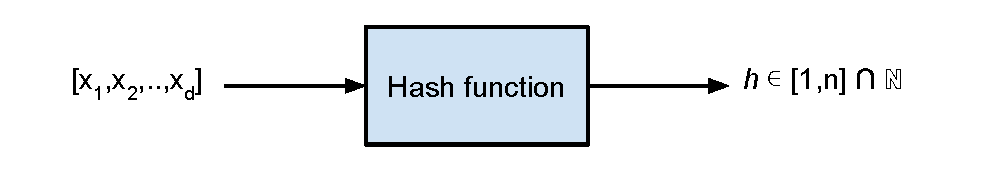
\includegraphics[scale=0.9]{images/hashing}
    \caption{Distributing the points based on a hash function}
    \label{fig:hashing}
\end{figure}

The main advantage of this approach is that if the hash function is known to all of the machines in the cluster and to all of the clients, point queries can be executed in O(1) network requests. Moreover, if the hash function is uniform, the multi-dimensional points are spread uniformly across the cluster, leading to a balanced storage load on all of the machines.

However, the use of a hash function for the point distribution presents some drawbacks. First of all, a hash function works well for a fixed number of hosts n. A different cluster configuration, with a different number of machines, requires the use of a different hash function. Moreover, changing the hash function requires a re-hashing of all of the points already stored in the cluster, potentially leading to a situation where all of the stored points need to be moved to a different machine. This situation would case a lot of traffic within the cluster, making it hard for the system to answer queries until the migration process is finished.

A second issue with use of hash functions is the observation that hash functions which are perceived to be good in this situation spread the multi-dimensional points uniformly across the machines in the cluster. In such a situation, is is quite likely that the hash function does not preserve point locality, and such, complex queries like range queries and nearest neighbour queries will need to be dispatched to all of the computing nodes in the cluster. 

\subsection{Spatial splitting}

Another approach that can be used for the point distribution problem is to partition the original space into a set of contiguous regions and assign each region to a host in the system. The most intuitive way to perform this split is to split the multi-dimensional space equally to obtain one region per index host. Figure \ref{fig:geometric-2hosts} shows a potential splitting of a 2D space for 2 hosts, while Figure \ref{fig:geometric-4hosts} presents a possible split of the same 2D space for 4 hosts. 

\begin{figure}[h]
\centering
\parbox{5cm}{
    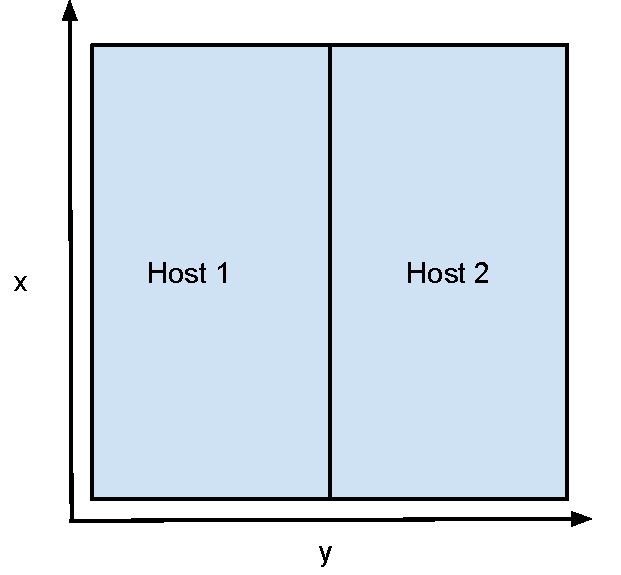
\includegraphics[width=5cm]{images/geometric-2hosts}
    \caption{Equal geometric space splitting for 2 hosts and 2 dimensions}
    \label{fig:geometric-2hosts}}
\qquad
\begin{minipage}{5cm}
    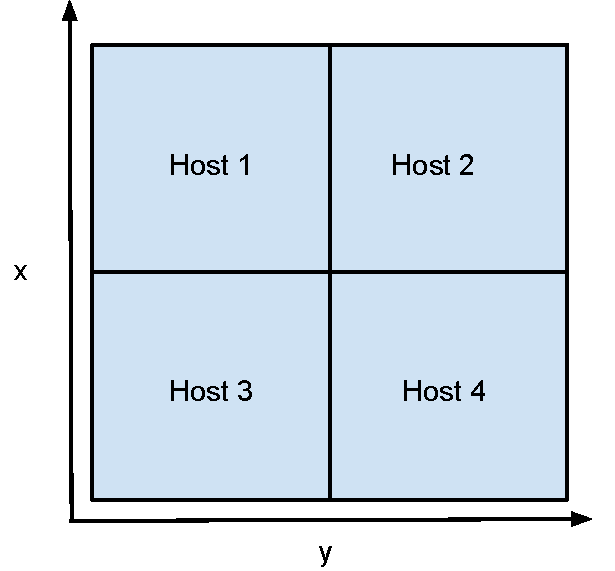
\includegraphics[width=5cm]{images/geometric-4hosts}
    \caption{Equal geometric space splitting for 4 hosts and 2 dimensions}
    \label{fig:geometric-4hosts}
\end{minipage}
\end{figure}

The spatial splitting approach is not only intuitive, but it also preserve locality, as generally, points which are close together are part of the same regions and are therefore stored on the same machine. Additionally, range queries can be resolved by dispatching the range query to all of the hosts whose assigned regions intersect with the range received as input. In the best case, range queries can be dispatched to a single host. It is generally preferable to split the space into hyper-rectangles, as these regions can be stored using only two data points, the bottom left and top right corners, independently of the number of dimensions of the original space. 

While the spatial splitting works well in some situations, sometimes it is unclear how to properly split the space between the machines. For example, the 2D space is easy to split into 2 or 4 equal regions, but it is more difficult to split for 3 or 5 hosts. It is always possible to split the space into n equal sized "strips", however this approach diminishes the locality of the data for large values of n. Representing regions as arbitrary polygons instead of hyper-rectangles addresses the problem to a degree, but storing these polygons and computing intersection between them is more difficult than performing the same task using hyper-rectangles. 

Difficulties in splitting the space can also arise even when using hyper-rectangle regions of different size. One instance is the case skewed point distributions, presented in figures \ref{fig:geometric-bad-split} and \ref{fig:geometric-bad-split-2}. In the case of the point distributions illustrated in these figures, an equal space partitioning would not split the points equally between the hosts. However, there are many possible rectangle-based splittings of the space, and it is unclear which of these it is better. In some case, the best split could be achieved by splitting the space into more regions than machines and assign each region to a machine.

\begin{figure}[t]
\centering
\parbox{5cm}{
    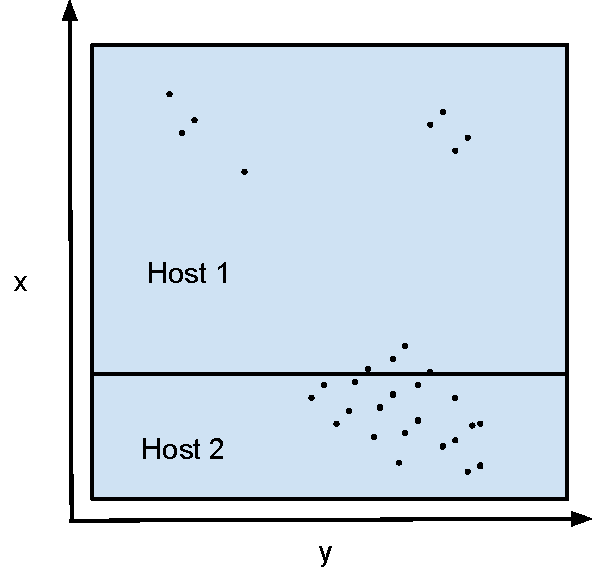
\includegraphics[width=5cm]{images/geometric-bad-split}
    \caption{Potential partitioning of the space for a skewed input distribution.}
    \label{fig:geometric-bad-split}}
\qquad
\begin{minipage}{5cm}
    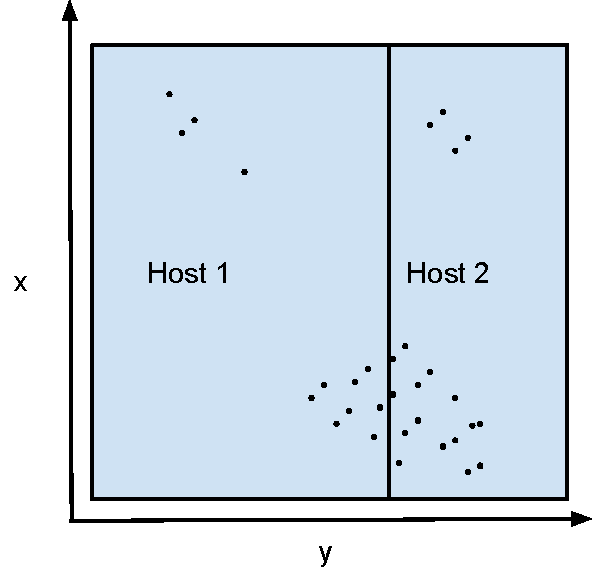
\includegraphics[width=5cm]{images/geometric-bad-split-2}
    \caption{Another potential partitioning for the same skewed input distribution.}
    \label{fig:geometric-bad-split-2}
\end{minipage}
\end{figure}
        
Additionally, in the case of skewed input distributions, the optimal split of the space into regions will change over time, as some regions will end up containing more and more points. In this case, the cluster needs to go through a \textit{re-balancing} phase, when the regions are modified and some points are moved from highly populated regions to less populated neighbouring regions. An important observation is that the number of neighbouring regions for an arbitrary region is a function of the number of dimensions of the original space. This leads to a large number of regions participating, or at least being considered, in the re-balancing of the points from a single dense region to its neighbours. 

\subsection{Z-Order curve splitting}

As previously mentioned, the in-memory PH-tree stores the multi-dimensional points according to the Z-ordering, by mapping the initial space to the 1-dimensional Z-order curve. This curve fills in the initial space in a contiguous and complete manner. Figure \ref{fig:zordering-clear}\footnote{Image adapted from \url{http://www.scholarpedia.org/article/B-tree_and_UB-tree}} shows the Z-order space filling curve filling the 2D space where the values in each dimension are limited by 3 bits.  

\begin{figure}[t]
    \centering
    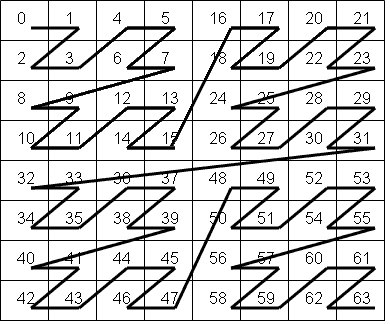
\includegraphics[scale=0.8]{images/zordering-clear}
    \caption{Z-order space filling curve filling the 2 dimensional space.}
    \label{fig:zordering-clear}
\end{figure}

Therefore, instead of splitting the original space into regions, one could attempt to partition the z-order curve into contiguous intervals. Figure \ref{fig:zorder-line} shows the 1 dimensional Z-order curve corresponding to the same 3 bit 2-dimensional space from figure \ref{fig:zordering-clear}, split into 4 intervals of different colours: $[{0, 12}]$ with blue, $[13, 35]$ with yellow, $[36, 47]$ with violet and $[48, 63]$ with green. Figure \ref{fig:zorder-square} shows how the interval splitting is reflected in the original space. Each interval on the Z-order curve corresponds to either a hyper-rectangle or a set of hyper-rectangles. For each interval there are at most $O(d*w)$ of these hyper-rectangles, where $d$ is the number of dimensions and $k$ is the number of bits needed to represented the values in each dimension. ~\cite{skopal2006-ubtree} provides an algorithm for generating the hyper-rectangles associated with a Z-order curve range.

\begin{figure}[t]
    \centering
\parbox{5cm}{
    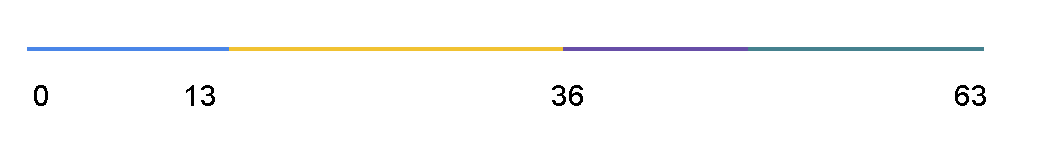
\includegraphics[width=5cm]{images/zorder-line}
    \caption{Example intervals on the 3bit Z-order curve}
    \label{fig:zorder-line}}
\qquad
\begin{minipage}{5cm}
    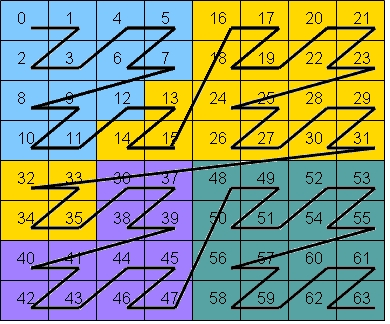
\includegraphics[width=5cm]{images/zorder-square}
    \caption{Example intervals on the 3bit Z-order curve filling the 2D space}
    \label{fig:zorder-square}
\end{minipage}
\end{figure}

An advantage of this splitting method is the regions corresponding to the Z-order intervals manifest locality, making it well suited for a point distribution method. Moreover, even if in the original space each region has $O(d)$ neighbours, each interval on the Z-order curve has a small, constant number of neighbouring intervals (2 for the interior intervals, 1 for the two edge intervals). This makes it easier to handle the cases in which a region is densely populated and should re-balance its points to neighbouring regions. 

Due to the presented advantages, the Z-order curve interval splitting is the method that was chosen as a point distribution strategy for the distributed PH-tree. 

\section{Architecture}
\label{sec:distindex-architectures}

The network architecture of the distributed PH-tree is presented in Figure \ref{fig:architecture}. The points are distributed to the hosts in the cluster using the Z-order curve interval splitting method. The \textit{key-mapping} is stored on the configuration server and is known to all of the nodes and the clients of the system. The configuration server uses a notification-based model and is responsible for notifying the indexing hosts and clients whenever any changes occur. This model reduces the amount of network traffic within the cluster, as nodes and clients only need to read the \textit{key-mapping} on start-up and do not need to poll the configuration server for changes. 

Clients of the index first connect to the configuration server, retrieve the \textit{key-mapping} and register to receive notifications if the mapping changes. After receiving the mapping, clients can begin to send queries to the indexing nodes within the cluster. Clients decide which hosts need to the contacted for a query based on the type of the query and the \textit{key-mapping}. This model is efficient as it allows the clients to decide the hosts to be queried based on local data. Furthermore, queries concerning more indexing nodes can potentially be executed by sending network requests in parallel to all of the involved nodes. A potential drawback of this model is that the configuration server could become the bottleneck in a system with many indexing hosts or many connected clients. This issue can be addressed by replicating the configuration data to a cluster of configuration servers. An alternative solution would be to store only a partial representation of the mapping in each indexing node and allow queries to be "hop" from one node to the other until they reach the destination machines, as in the case of the previously discussed distributed hash tables. However, the extra latency introduced by repeated "hops" with the cluster makes this approach ill-suited for latency-sensitive applications like a distributed-index.  

\begin{figure}[t]
    \centering 
    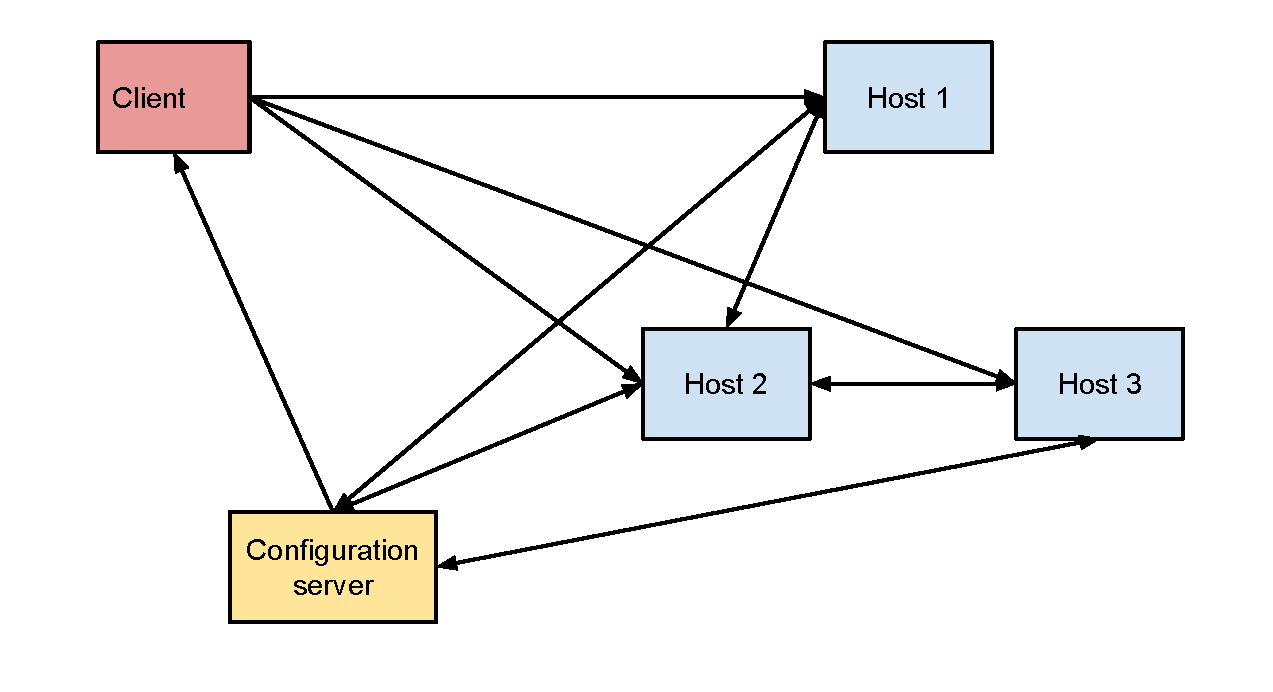
\includegraphics[scale=0.6]{images/architecture}
    \caption{The network architecture of the distributed PH-tree}
    \label{fig:architecture}
\end{figure}

As the data is split according to Z-order curve intervals, each indexing hosts only needs to maintain two connections to other hosts in the cluster (or 1 for the hosts holding the edge intervals). This means that the amount of memory used by the hosts to store cluster membership information remains relatively constant, even if the number of the nodes in the cluster increases. 

\section{Algorithms}
\label{sec:distindex-algorithms}

This section will discuss how the \textit{key-mapping} is created from the Z-order curve intervals and how the queries are executed based on the key-mapping. 
\subsection{Key-mapping design}
\label{sec:distindex-key-mapping}

The \textit{key-mapping} used by the distributed PH-tree assigns the points based on the Z-order curve intervals. To determine the host responsible for a certain multi-dimensional point, one would have to map that point to the Z-order curve and determine the interval that contains it. There are two alternative for designing the \textit{key-mapping} based on the Z-order curve intervals:
\begin{enumerate}
    \item Store the Z-intervals directly as pairs of Z-values and perform 1-dimensional interval matchings to determine the hosts that have to be contact for certain queries. The operation is linear in the number of hosts, for both point and range queries, as the Z-values of the query points need to be compared with the Z-values of the intervals. The correctness of this approach stems from the fact that the region represented by a $d$-dimensional hyper-rectangle [X, Y] \footnote{Where X is the top-right corner of the hyper-rectangle and Y is the bottom-left corner of the hyper rectangle} is included in the set of d-dimensional regions corresponding to the Z-interval $[Z_X,Z_Y]$.
    \item Store the hyper-rectangles from the original space that correspond to each Z-order interval and perform intersections between the query points/rectangles from the original space and the hyper-rectangle of the interval regions. The complexity of this operation is $O(n * w * d)$, as each region contains at most $O(w * d)$ hyper-rectangles. 
\end{enumerate}

Even if the first solution is asymptotically faster than the second one for finding the hosts to query, the first approach attempts to query a much larger area in the original space than the second one. Therefore, the first method can potentially generate many more network requests than the first one, especially in a system with a large number of online indexing hosts. Moreover, the intersection operation itself is performed on the client, in-memory, and does not generate a network request. Because of these reasons, the second approach is preferable to the first approach in a system looking to minimize the number of network requests associated to each query, like the distributed PH-tree. 

\cite{skopal2006-ubtree} presents an algorithm to decompose a Z-order interval into a set of at most $O(w*d)$ rectangles. These rectangles are then stored in a multi-dimensional data structure providing hyper-rectangle intersection operations.\footnote{This implementation actually uses a variant of the in-memory PH-tree for this function.}

\subsection{Point operations}
Point operations involve a single query point, like the insertion or removal of a key-value pair, obtaining the value associated with a key value pair or changing the key associated with a key-value pair. For the point queries, the client only needs to determine which host to send the request to. This is done by determining the intersections between the query point and the hyper-rectangles corresponding to the Z-order intervals. In the case of the \textit{get()}, \textit{put()} and \textit{delete()} operations, the client sends the request to the hosts responsible for the query point and returns the result of the operation. In the case of the \textit{updateKey()} operations, it is possible that a different host is currently responsible for the new key of the value associated with the query point. In that case, the \textit{updateKey()} operation is performed in two steps: first the client removes the old key from the host responsible for it, and the inserts the new key to the proper host.

\subsection{Range queries}

Range queries have the form \textit{range\_query(bottom-left, top-right)}. Both of the received arguments are multi-dimensional data points and this operation returns all of the points in the index that fall inside the multi-dimensional rectangle defined by these two points. These operations are resolved in the following manner on the client. First, the client performs an intersection between the hyper-rectangle range and the hyper-rectangles associated with the Z-order intervals contained in the \textit{key-mapping}. It then send requests to all of the hosts whose regions were intersected, receives and combines the results. It is important to note that each host returns a list of point that are already ordered via Z-ordering and because the nature of the Z-order interval split, these lists do not need to be merged, but only concatenated.

A range query can generate up to $O(n)$ network requests, as in some cases, all of the hosts might need to be contacted. However, as previously also mentioned in section \ref{sec:distindex-key-mapping}, the \textit{key-mapping} performs the intersection between the query-rectangle and the regions corresponding to the Z-order intervals, instead of performing the intersection between the Z-order interval of the query range and the Z-order intervals of the machines. This guarantees that hosts which \textit{cannot} contain points in the query range will not be queried. It is however possible that some hosts will not contain any points falling in the query hyper-rectangle, even if the regions they are responsible for intersects with the query range.

\begin{figure}[t]
    \centering
    \begin{subfigure}[b]{0.4\linewidth}
        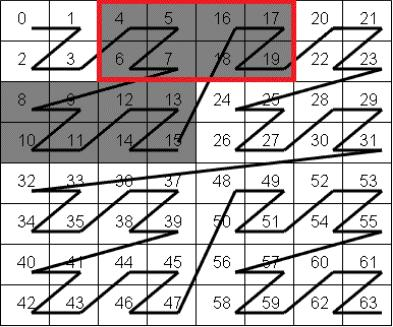
\includegraphics[width = \linewidth]{images/zordering-range}
        \caption{The 2-dimensional range $[(0, 2), (1, 5)]$ overlaid on the Z-order curve.}
        \label{fig:range-zorder}
    \end{subfigure}%
    \qquad
    \begin{subfigure}[b]{0.4\linewidth}
        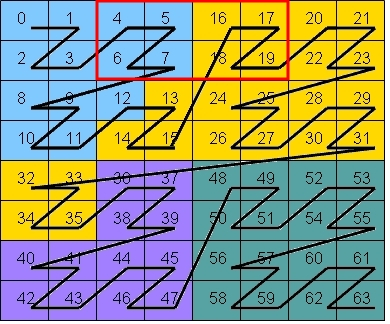
\includegraphics[width = \linewidth]{images/zordering-range-intervals}
        \caption{The intervals specific in the previous section overlaid over the previous picture.}
        \label{fig:range-zorder-intervals}
    \end{subfigure}
    \caption{Illustration of a range query intersected with the host intervals}
    \label{fig:range}
\end{figure}

Figure \ref{fig:range-zorder} illustrates an example range query. It shows the range defined by the bottom left point $[(0, 2)]$ and top right point $[(1, 5)]$ overlaid against the 3-bit Z-order curve. The Z-order interval corresponding to this range is $[4, 19]$ and the 2 dimensional region associated to it includes the $[(0, 2), (1, 5)]$ rectangle. Figure \ref{fig:range-zorder-intervals} also displays the regions associated to each host according to the split presented in Figure \ref{fig:zorder-line}. In this case, only the hosts responsible for the blue and yellow regions need to be contacted by the client. 

As previously mentioned, because the Z-order range associated with the query range corresponds to a larger regions than the query hyper-rectangle, especially in high dimensional spaces, 

\subsection{Nearest neighbour queries}

Nearest neighbour queries return the $k$ nearest points, according to the Euclidean distance, to an arbitrary query point, thus having the form \textit{knn\_query(q, k)}. The query point does not need to be stored in the index. The execution of a nearest neighbour query has the following steps:
\begin{enumerate}
    \item The client first determines which hosts is responsible for the query point $q$ and forwards the query to this host.
    \item After receiving the result, the client determines the furthest neighbour $fn$ of the query point $q$ according to the Euclidean distance. 
    \item The client computes the distance $d = dist(q, fn)$ and performs a range query on the range $[q - d, q + d]$ .
    \item The final result of the nearest neighbour query consists of the $k$ points from the result of the previously executed range query that are closest to $q$.  
\end{enumerate}

The additional range query is needed because the Z-order splitting, or any other geometrical splitting, does not guarantee that closest $k$ neighbours of a point will be placed in the same regions as the point itself. This range query ensures that points which are closer to $q$ than $fn$, but stored in a different region, will also be returned. 

It is sometime possible that the initial query sent to the host responsible for $q$ will return fewer than $k$ points. This will generally only happen when the cluster contains very few points. In this case, the queried area should be iteratively increased until at least $k$ points are returned. This can be done by computing the distance $d$ and iterative increasing it until the range query $[q - d, q + d]$ returns at least $k$ points.

\begin{figure}
    \centering
    \begin{subfigure}[b]{0.4\linewidth}
        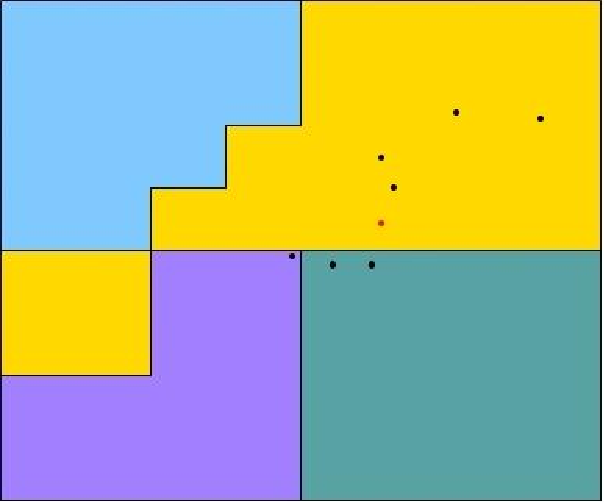
\includegraphics[width = 2.5in]{images/zordering-knn-a}
        \caption{The 2 dimensional space.}
    \end{subfigure}%
    \qquad
    \begin{subfigure}[b]{0.4\linewidth}
        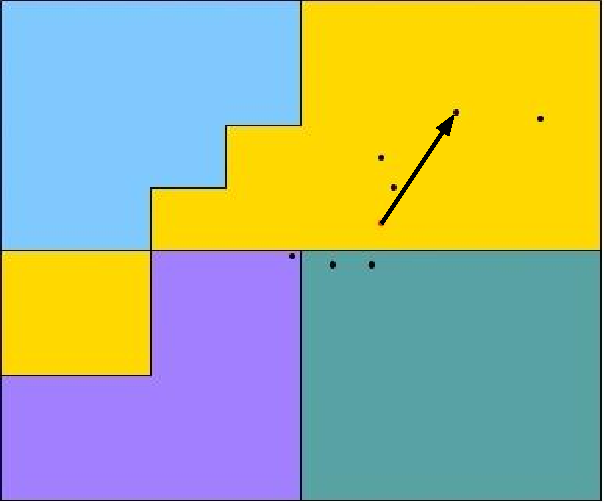
\includegraphics[width = 2.5in]{images/zordering-knn-b}
        \caption{Distance to further neighbour.}
    \end{subfigure}
    \begin{subfigure}[b]{0.4\linewidth}
        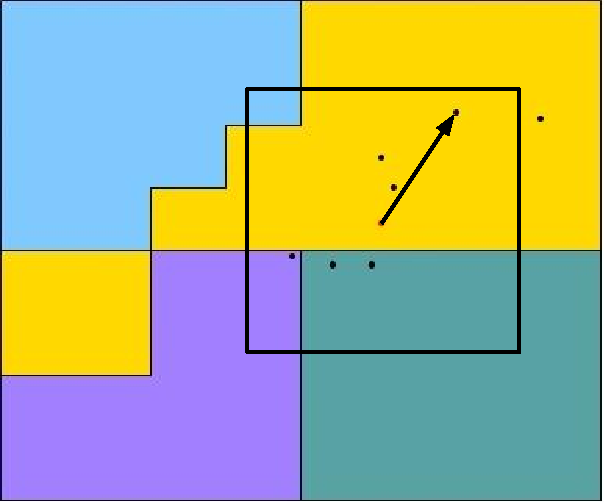
\includegraphics[width = 2.5in]{images/zordering-knn-c}
        \caption{The additional rectangle range query.}
    \end{subfigure}%
    \qquad
    \begin{subfigure}[b]{0.4\linewidth}
        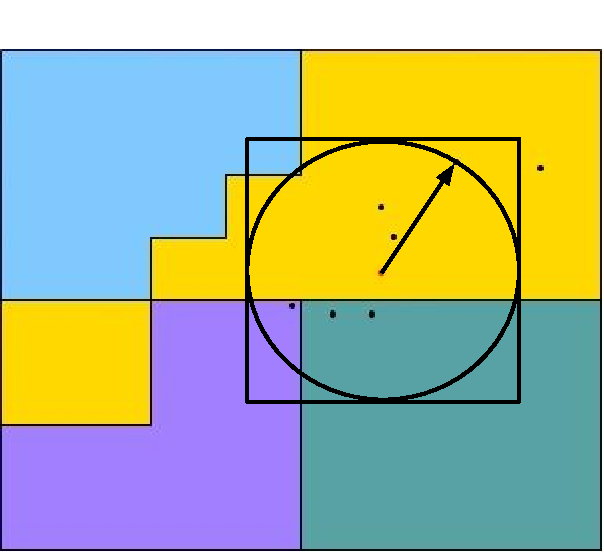
\includegraphics[width = 2.5in]{images/zordering-knn-d}
        \caption{The optimal circle range query.}
    \end{subfigure}
    \caption{Illustration of a 3 nearest neighbour query execution in a 2 dimensional space. }
    \label{fig:knn}
\end{figure}

While this approach for finding the $k$ nearest neighbours of a query point is correct, it is not the most efficient one. The main issues is that the additional range query searches for other neighbours in a hyper-cubing range. The optimal strategy would be to search for these neighbours in hyper-sphere of radius $d$ centered at $q$. This circle is inscribed in the hyper-cube search by the range query, as illustrated in Figure \ref{fig:knn}d. Therefore, the algorithm presented in this work can sometimes send unnecessary request to hosts responsible for the areas outside of the circle and still within the hypercube. This is generally not a problem in lower dimensional spaces, however the different in volume between the hyper-cube and the hyper-sphere increases gradually with dimensionality of the space. 

\subsection{Entry load balancing}

As previously described, data sets which are skewed towards certain areas of the multi-dimensional space will cause some machines to store more points than the others. A load balancing algorithm is needed to balance the amount of entries stored across the cluster, such that each hosts stores roughly the same amount of entries. 

Each host is assigned a threshold $t$ corresponding to the maximum number of entries it can store. For simplicity, we assume that all the hosts in the system are identical and have the same $t$. The load balancing algorithm used by the distributed PH-tree assumes that values stored with each data points have roughly the same size, and such a threshold on the number of entries a hosts can store coincides with the amount of data it can store. The presented balancing algorithm can easily be modified by simply using the amount of occupied memory as a threshold. 

Furthermore, the configuration server maintains the number of entries associated to each hosts, which will be referred to as the \textit{size} of the host. To improve scalability, the hosts do not update the size stored in the configuration server after each individual write operation, but only after a certain number of write operations were performed since the last update. An alternative solution would be update the size at a fixed time period. Each host maintains a cached copy of the size information, and is notified by the configuration server when a different host updates this information.

After the number of entries stored by a certain host reaches the balancing threshold $t$, that host will attempt to move some of the points it stores to a neighbouring host. This process is referred to as a \textit{re-balanacing operation} and will change the Z-order intervals of both the host initiating the re-balancing and the host receiving the additional entries.
Given a host $h$ responsible for an arbitrary interval, the host responsible for the Z-order interval to the right will be called its \textit{right neighbour}. Similarly, the host responsible for the Z-order interval to the left will be called the $h$'s \textit{left neighbour}. 

The re-balancing algorithm proceeds as follows: 
\begin{enumerate}
    \item The \textit{initiator} host checks the size of the hosts responsible for the intervals to the left and to the right of its Z-order interval. When the host responsible for the leftmost intervals initiates a re-balancing operation it only checks the size of its right neighbour, while the host responsible for the rightmost interval only considers re-balancing to its left neighbour.
    \item The \textit{initiator} selects the neighbouring host with the fewest entries and sends an initiate balancing message. If the neighbour is available to participate in the operation, the algorithm continues with the following step. If the neighbour is busy, the \textit{initiator} will attempt to re-balance to the other neighbour. If that is not possible, the re-balancing operation fails and will be re-attempted at a later point.
    \item The initiator sends a subset of its entries to the \textit{receiver} host. This subset is a contiguous run of entries stored by the initiator.
    \item After the entries have been moved, the \textit{initiator} updates the \textit{key-mapping} on the configuration server. 
    \item The initiator sends a commit message to the \textit{receiver} host, notifying it that the operation was successful. After this message is sent, both hosts mark themselves as available for any other re-balancing operations.
\end{enumerate}

This algorithm allows a host $h$ to be part of only a single re-balancing operation at a moment in time. As soon as a host successfully initiates a re-balancing operation, both the \textit{initiator} and the \textit{receiver} mark themselves as busy and will refuse further re-balancing initiation operations until the current operation is finished. This allows up to $n/2$ balancing operations to run in parallel across the cluster, as each operation involves two neighbouring hosts.

Furthermore, clients currently balancing do not accept write requests. This is done to prevent the \textit{initiator} host to accept updates to the section of Z-order curve that is currently re-balanced to the \textit{receiver} host.

\chapter{Concurrency}
\label{ch:concurrency}

\section{Challenges}
The first version of the PH-tree does not support concurrent access, and remains consistent only if accessed by a single thread at a time. With the current popularity of multi-core CPU's, concurrent access has the potential of providing a significant improvement in the throughput of the PH-tree. The addition of concurrent access presents the following challenges:
\begin{itemize}
    \item Concurrent access strategies must guarantee that PH-tree remains consistent for any number of threads that access it and for any arbitrary interleaving of the executions of these thread. Furthermore, deadlock should not occur when the data structure is accessed by multiple threads.
    \item The chosen strategy should optimize the execution time for the most common operation, by minimizing for example, the amount of locks that have to be taken during for those operations. In case of an indexing data structure, read operations are more common than write operations and should be prioritized by the concurrency strategy from the response time point of view.
    \item Different concurrent access strategies come with different consistency guarantees. For example, consider the situation in which two processes A and B work concurrently on a shared data structure. Process A starts a read operation at time $t$ and process B a write operation at time $t + \epsilon$. The consistency model determines if process A might see the changes made by process B, if process B finishes the operation before A.
    \item The PH-tree also supports an iterator over all of the entries or over all of the entries contained within a specified hypercube. The concurrency strategy should allow iterators to traverse a PH-tree, even if the tree is concurrently modified by other threads. The concurrency model corresponding to the concurrency strategy used will specify which entries of the tree are seen by the iterator.
\end{itemize}

\section{PH-tree structure}

The PH-tree stores key-value pair entries. The keys are multi-dimensional data points and the values are optional. The entries are stored as bit strings, to exploit any prefix sharing between the bit strings of the keys and reduce the storage requirements. 

Figure \ref{fig:phtree-node-1} illustrates a 2 dimensional PH-tree containing  the entries (0000, 1000), (0011, 1010), (1011, 1000). Figure \ref{fig:phtree-node-2} shows the corresponding node structure for the same PH-tree. Each node contains a \textit{prefix}, a \textit{a hypercube} (HC) and a set of \textit{postfixes}. The \textit{prefix} is a portion of the bit string common to all bit string portions stored in that node. A \textit{postfix} is an ending portion of a single bit string. The \textit{hypercube} is a data structure that stores references to \textit{postfixes} or subnodes. Currently, the PH-tree supports multiple representation for the \textit{hypercube}, either as an array (HC) or a sparse linear representation {LHC}. For example, the root node in Figure \ref{fig:phtree-node-1} has a \textit{hypercube} storing references to two subnodes. The subnodes each have an associated \textit{prefix} and a \textit{hypercube} storing links to postfixes. 

This structural representation of the PH-tree has the following important consequences:
\begin{itemize}
    \item All information stored in a node cannot be read or written in an atomic manner, as the prefix, the hypercube and the postfixes need to be read or written in separate instructions. 
    \item Adding a new subnode to a node, as well as removing or replacing it can be done atomically.      
\end{itemize} 

\begin{figure}
    \centering
    \begin{subfigure}[b]{0.6\linewidth}
        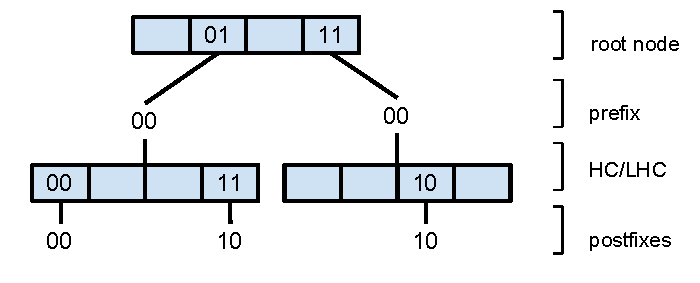
\includegraphics[scale=0.7]{images/PH-tree-nodes}
        \caption{Logical structure of a PH-tree.}
        \label{fig:phtree-node-1}
    \end{subfigure}%
    \begin{subfigure}[b]{0.4\linewidth}
        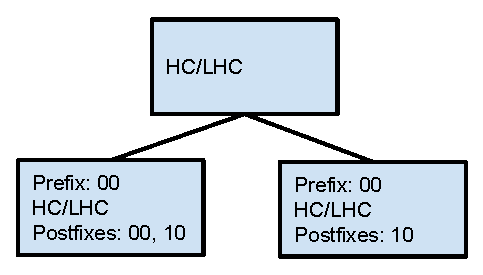
\includegraphics[scale=0.7]{images/PH-tree-nodes-2}
        \caption{Node structure of the same PH-tree}
        \label{fig:phtree-node-2}
    \end{subfigure}
    \label{fig:phtree-nodes}
    \caption{A 2 dimensional PH-tree containing three 4-bit entries: (0000, 1000), (0011, 1010), (1011, 1000). The values are omitted. }
\end{figure}

The following section presents the concurrent access strategies added to the PH-tree and discusses their consistency guarantees.
\section{Concurrency strategies}

\subsection{Copy-on-Write}

Copy-on-Write is an concurrent access strategy that allows multiple threads to access the same shared data structure. When one of these threads needs to modify the shared data structure, it first makes a copy of it, performs the modifications and then updates it with its modified copy. Each write operation creates a new version of the shared data structure, making it immutable. This strategy allows one writer thread and an arbitrary number of reader threads to work on the same data in the same time. If multiple writer threads were to access the data structure, each would end up with its updated copy and the last to replace the shared data structure with the copy would overwrite the changes of the other writer. 

In case of the trees, writer threads do not have to copy the full tree before applying their modifications. It is sufficient to create a copy of the node that is updated and copies of all of its ancestor nodes, up to and including the root of the tree. The number of nodes copied for each update is equal to the maximum height of the tree. In case of the PH-tree, this number is equal to the number of bits needed to represent the values on each dimensions, independent of the number of nodes or entries currently stored in the tree. 

Figure \ref{fig:tree-cow} illustrates the execution of write operation. For simplicity, a general binary tree is pictured here, as the operation is executed in a similar manner on a PH-tree. In this example, node G needs to be updated. To achieve this, all of the ancestors of G are copied and the copy of G, $G'$ is updated. Finally, the root pointer of the tree is changed from A to $A'$ atomically. It is important that the root swap is performed in an atomic manner, such that any readers concurrently accessing the tree will either access the old or the new version of the tree.

\begin{figure}[h]
    \centering 
    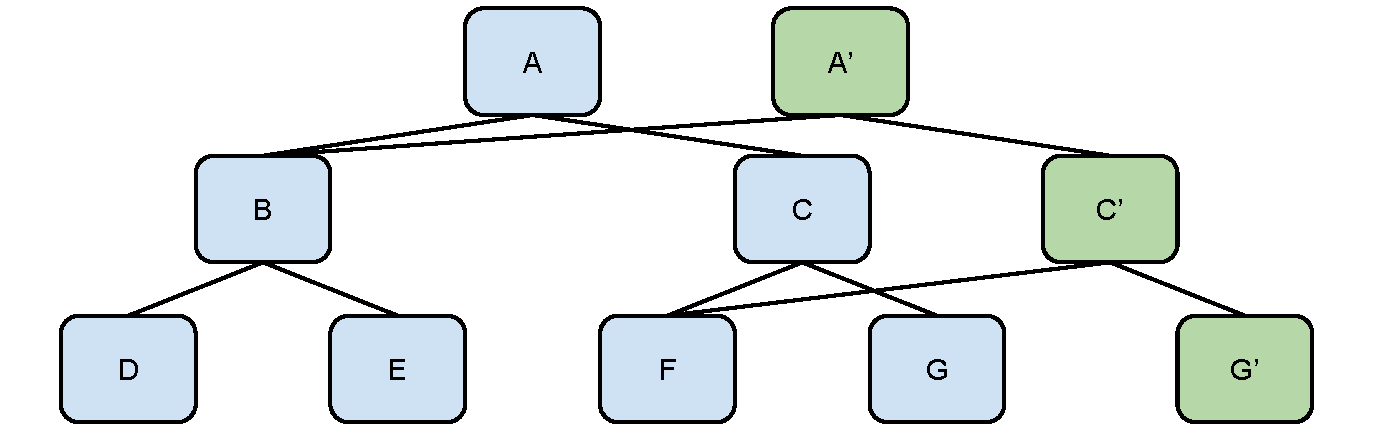
\includegraphics[scale=0.6]{images/Tree-COW}
    \caption{Illustration of Copy-on-Write on a binary tree where the node G has to be written}
    \label{fig:tree-cow}
\end{figure}

There are several possibilities to handle multiple writer threads using the Copy-on-Write strategy. One approach would be allow multiple threads to access the tree in the same time. This can be done by implementing the atomic root swap using a Test-And-Set atomic operation, essentially turning each write operation into a transaction. In case the root was changed since the thread has started the operation, the atomic Test-And-Set fails and the thread will need to restart the operation. The main drawback of this approach is that the commit fails even if the changes are made to different parts of the tree.

Iterators created on a Copy-on-Write PH-tree essentially traverse a snapshot of the tree taken on the iterator creation time $t$. If an iterator is create at time $t$, it will view all of the entries that were contained in the tree at time $t$, even if these entries were removed from the tree before the iterator finishes. Moreover, iterators will never see any entries that may have been added to the PH-tree after time $t$.

\subsection{Locking}

A very simple way to handle concurrent writer threads is to use a global lock that each thread must take before the execution of an operation. If the lock is a mutex, the tree can only be accessed by a single thread, and if the thread is a read-write lock, the tree can be accessed by either a single writer or several reader threads. This coarse-grained locking strategy is not very efficient and therefore only useful as a baseline implementation during the performance evaluation.

\textit{Fine grained} locking strategies perform locking at the level of tree nodes and can allow multiple writer threads to modify the tree in the same time. Two popular strategies are described in the following sections.  

\subsubsection{Hand-over-Hand locking}

\begin{figure}[t]
    \centering
    \begin{subfigure}[b]{0.5\linewidth}
        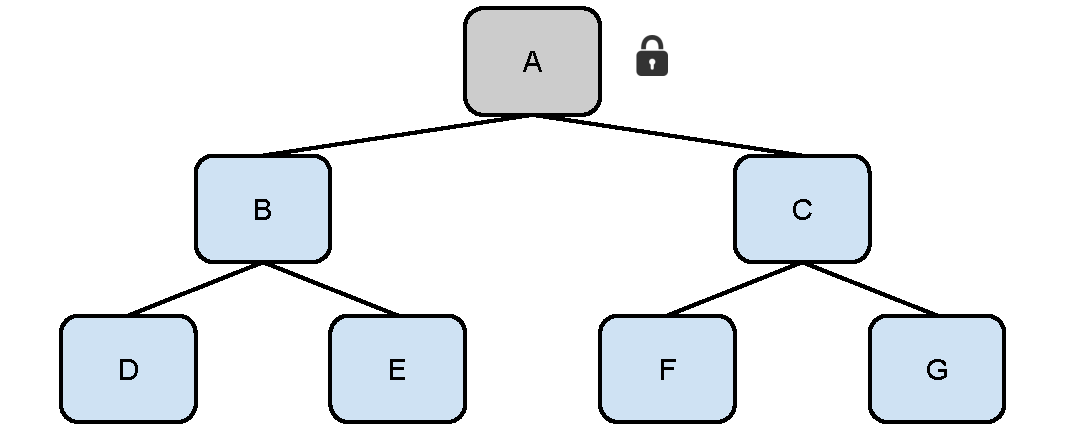
\includegraphics[width = 3in]{images/Tree-HoH-a}
        \caption{The root is locked}
    \end{subfigure}%
    \begin{subfigure}[b]{0.5\linewidth}
        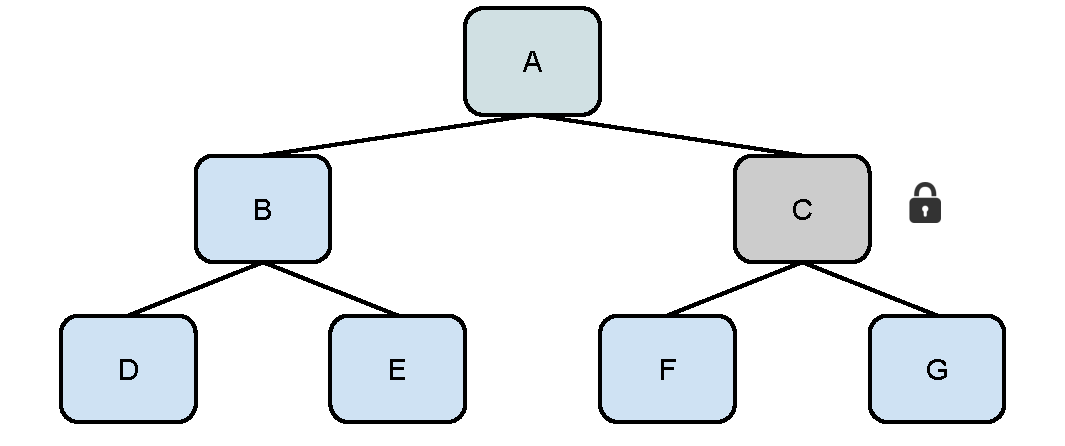
\includegraphics[width = 3in]{images/Tree-HoH-b}
        \caption{The next node is locked}
    \end{subfigure}
    \begin{subfigure}[b]{0.5\linewidth}
        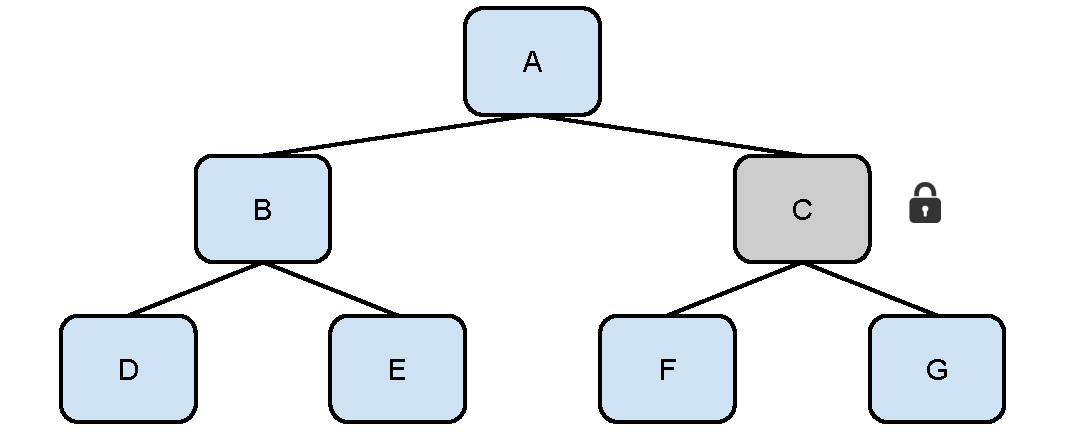
\includegraphics[width = 3in]{images/Tree-HoH-c}
        \caption{The root can now be unlocked}
    \end{subfigure}%
    \begin{subfigure}[b]{0.5\linewidth}
        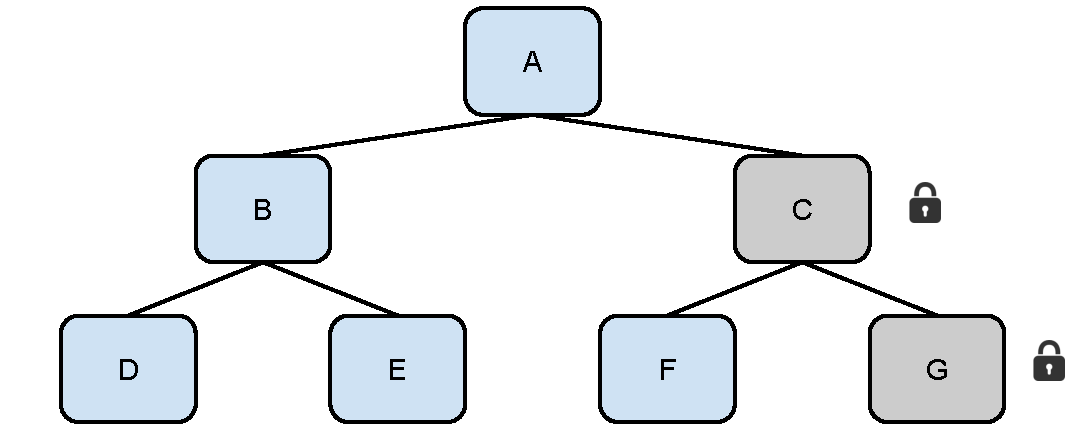
\includegraphics[width = 3in]{images/Tree-HoH-d}
        \caption{The final node is locked}
    \end{subfigure}
    \caption{Illustration of hand-over-hand locking descent to node G}
    \label{fig:locking-hoh}
\end{figure}

Hand-over-hand locking, also called \textit{lock-coupling}, is a fine-grained locking strategy according to which a lock for a node can only be acquired if the parent lock is also held. When traversing the tree according to this strategy, at most two lock will be held by a thread at a time. An additional lock needs to be acquired before acquiring the lock of the root of the tree, to prevent conflicts on the creation of the first node of the tree. 

Figure \ref{fig:locking-hoh} shows the sequence of events happening when a thread needs to update a node. The node to be updated in this figure is node G. The thread first acquires the root, descends to node C and acquires that lock as well. The root can be unlocked before descending to node G and acquiring that lock. After the changes are done, the lock of node G is unlocked.

This strategy allows multiple threads to modify the different subtrees of the tree. The main drawback of this approach is that if the non-leaf nodes are modified, subtrees of those nodes cannot be modified of a different thread until the current thread finishes the update operation. Secondly, there will be a high contention for the locks on the higher levels of the tree, which could negatively affect performance for write-heavy workloads. 

\subsubsection{Optimistic locking}

\begin{figure}
    \centering
    \begin{subfigure}[b]{0.5\linewidth}
        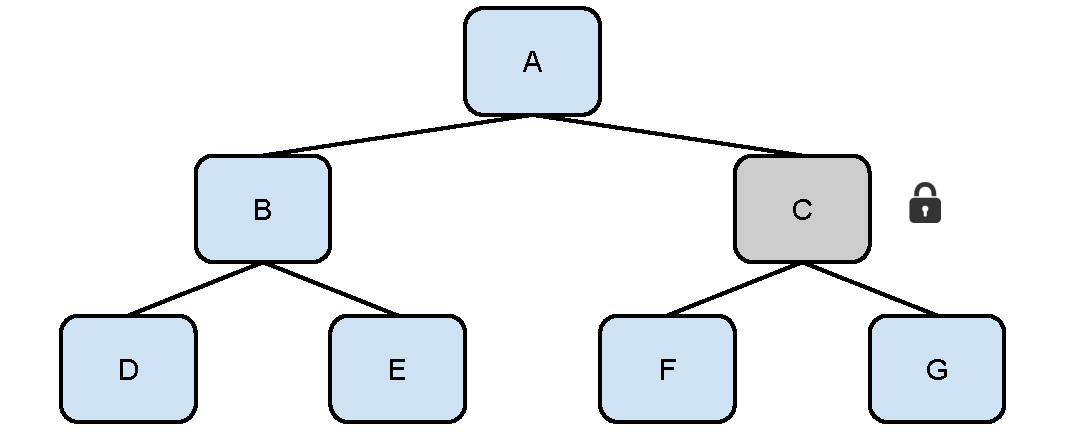
\includegraphics[width = 3in]{images/Tree-HoH-c}
        \caption{The parent of the target node is locked}
    \end{subfigure}%
    \begin{subfigure}[b]{0.5\linewidth}
        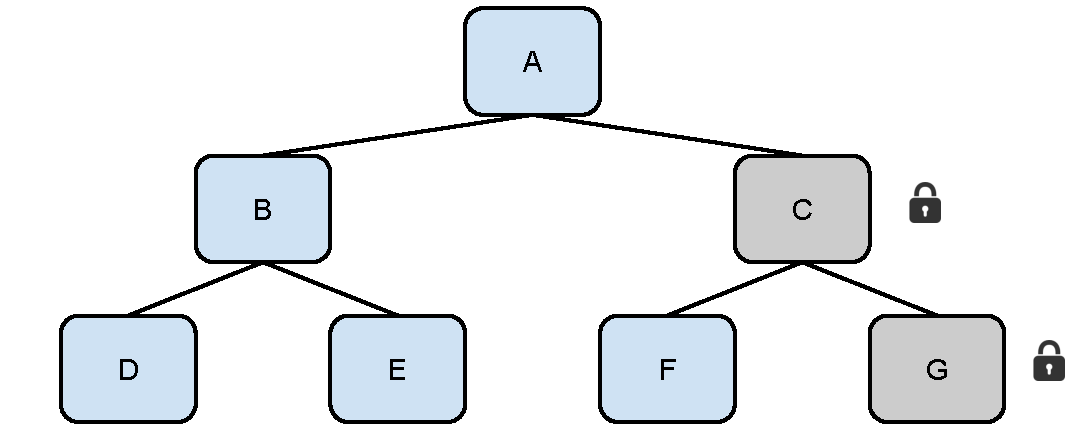
\includegraphics[width = 3in]{images/Tree-HoH-d}
        \caption{The target node is locked}
    \end{subfigure}
    \caption{Illustration of optimistic locking descent to node G}
\end{figure}

Optimistic locking is an alternative fine grained locking strategy which seeks to minimize the number of locks which are take during a write operation. The basic idea is to traverse the tree without acquiring any locks until the node to be updated is reached. Once at the target node, the writer thread acquires the lock of the parent and the lock of the current node. After this happens, the write operation can continue only if both of these two nodes have not yet been removed from the tree and the current node is still a child node of the parent node. If any of these checks fail, the write operation fails and the current thread begins another attempt by starting a new traversal of the tree.

To speed up checking if a node is still reachable from the root nod, each node has an additional removed flag, which indicates if certain node has been removed from the tree. When a thread removes a node, it sets this flag to true before releasing the lock of the node. 

One advantage of this method is that in a large tree, re-tries are generally rare as threads do not generally attempt to update the same node. Moreover, a thread holding the lock of a certain node does not block other threads from performing update operations on the node's subtrees, unlike the \textit{hand-over-hand} strategy.

It is important to mention the fact the in the case of the PH-tree, all update operation to a single node are not executed in an atomic fashion, which can cause reader threads to perform reads from nodes which are in an inconsistent state. This can be avoided by protecting the nodes with a read-write lock and requiring the read operations to acquire the read lock of a node before performing a read. However, the latency of the read operation is increased if readers need to acquire locks. Another solution is to add some copy-on-write logic to the write operations. Specifically, before performing a write operation on certain node, the writer thread first creates of copy of the node, performs the update on the copy and then atomically replaces the parent node's reference to the node with the copy. As the writer thread holds the lock on the parent node, it is guaranteed that no other writer threads will overwrite this change. Furthermore, reader threads will either access the old version of the node or the updated copy, as the sub node swap is done in an atomic manner.

In the case of the fine-grained locking concurrency strategies, iterators running the PH-tree operate according to a relaxed consistency semantics. Therefore, an iterator created at time $t$, which finished traversing the tree at time $e$ will see all of entries that were part of the tree a time $t$ and are still part of the tree at time $e$. Moreover, entries inserted or removed in the time interval $[t, e]$ may also be seen by the iterator. It is however guaranteed that all of the entries seen by the iterator are visited according the Z-ordering. 

The PH-tree supports both a full COW concurrency strategy and the fine grained locking strategies. The optimistic locking strategy is generally faster than the hand-over-hand locking strategy, but can lead to starvation when many threads need to update the same node or nodes which are close together. The choice between the COW strategy and the fine grained strategies comes down to the choice between the consistency guarantees provided by them. For example, snapshots of the tree can only be obtained if the tree is using the COW strategy. 

\chapter{Implementation}
\label{ch:implementation}

\section{System architecture}

The architecture of the distributed PH-tree is shown in Figure \ref{fig:implementation-architecture} . The implementation consists of two artifacts: the \textit{client library} and the \textit{middleware library}. Both of these libraries have been implemented in the Java programming language and are the main artifacts of this work.

\begin{figure}[h]
    \centering 
    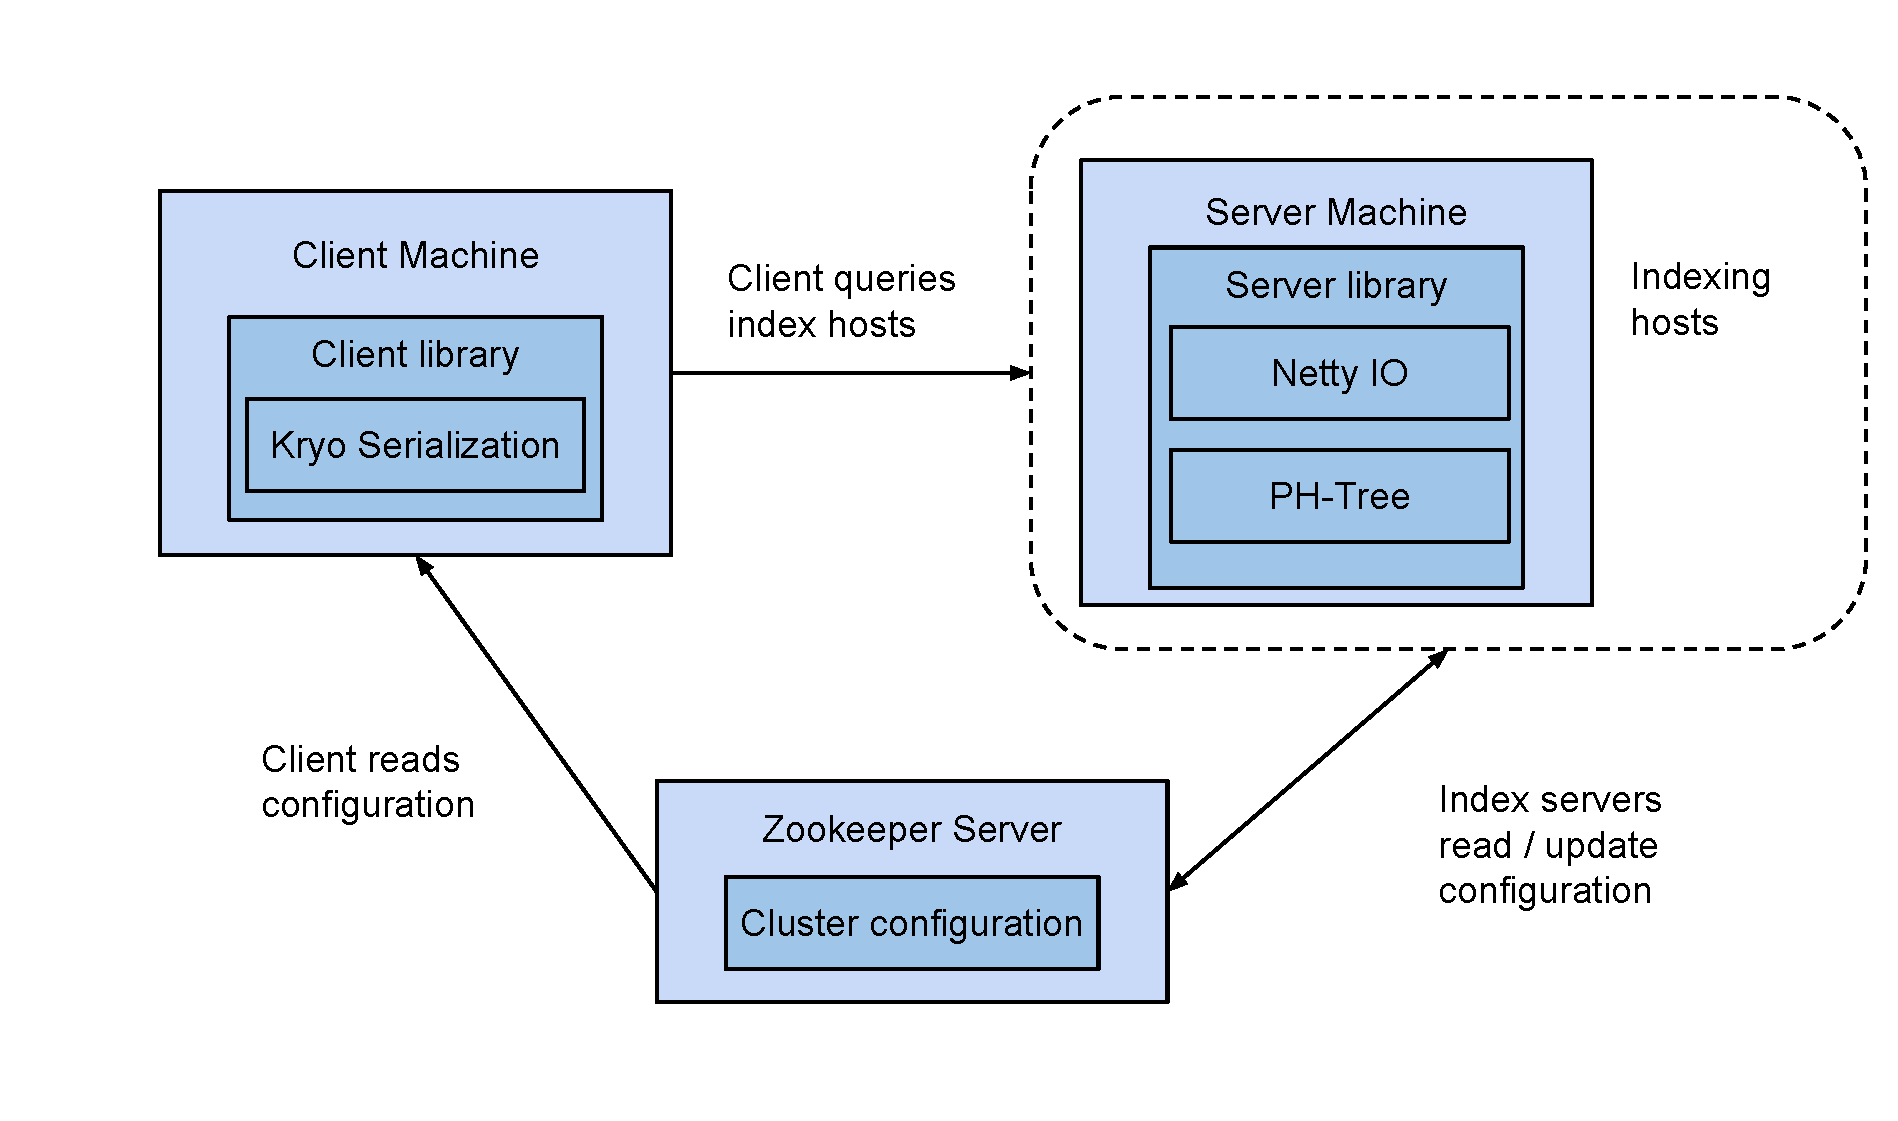
\includegraphics[scale=0.4]{images/implementation-architecture}
    \caption{The implementation architecture of the distributed PH-tree}
    \label{fig:implementation-architecture}
\end{figure}

The \textit{client library} is deployed on the clients and contains the code necessary to connect to the configuration server, retrieve the cluster information and perform operations on the cluster. The \textit{client library} also contains a dependency to the \textit{Kryo} library, a Java serialization library that used to encode the values stored on the PH-tree before performing to the insertion operation and decode the values retrieved from the server. Clients cannot modify the cluster information and can only subscribe to be notified by the configuration server when indexing hosts join or leave the cluster and when the Z-order curve intervals changes as a result of a rebalancing operation.

The \textit{server library} contains the index middleware logic and needs to be deployed on the indexing hosts. The \textit{server library} implements a multi-threaded middleware Java application running on the indexing hosts. The \textit{Netty IO}\footnote{http://netty.io/} library is used to handle incoming client requests using a thread pool. When a server is started, it first connects to configuration server to retrieve the cluster information and then is assigned an interval of the Z-ordr curve for which it is responsible. If the cluster alredy contains some data the new node can join mark itself as a free node and will be contacted by the next node in the cluster that will begin a balancing operaton. Indexing hosts update the intervals in the cluster configuraton after a balacin operation and periodically update the number of entries stored. 

The \textit{configuration server} was implemented using \textit{ZooKeeper}\footnote{http://zookeeper.apache.org/}, an open source server whose goal is to provide reliable distributed coordination. Zookeeper provides a centralized service for maintaining configuration information and performing distributed synchronization. The \textit{cluster configuration} is stored is a ZooKeeper specific format by the indexing hosts. ZooKeeper also allows the possibility of replicating the stored configuration by running a \textit{qourum}\footnote{The name used by ZooKeeper for a replicated cluster of ZooKeeper server.} of machines to improve availability. 

A minimal configuration of the distributed PH-tree requires a ZooKeeper server, an indexing host running the \textit{server library} and client machines performing operation using the \textit{cluster library}.

\section{PH-tree Java API}

The Java API of the PH-tree is presented in Figure \ref{fig:PH-tree-Java-API}. The interface \textit{PhTreeV} is the main interface and corresponds to a PH-tree that stores entries with keys of type \textit{long[]} and arbitrary objects as values. A set API is provided through the classes \textit{PhTree} and \textit{PhTreeD}. \textit{PhTree} uses a \textit{PhTreeV} instance with empty values to implement a set for multi-dimensional points with values of type \textit{long}. \textit{PhTreeVD} is targeted towards application which require floating point precision for the values of each dimension. This type of tree is backed by the \textit{PhTreeV} instance and performs pre and post processing of the multiple-dimensional points to map them from \textit{double[]} to \textit{long[]}.

\begin{figure}[h]
    \centering 
    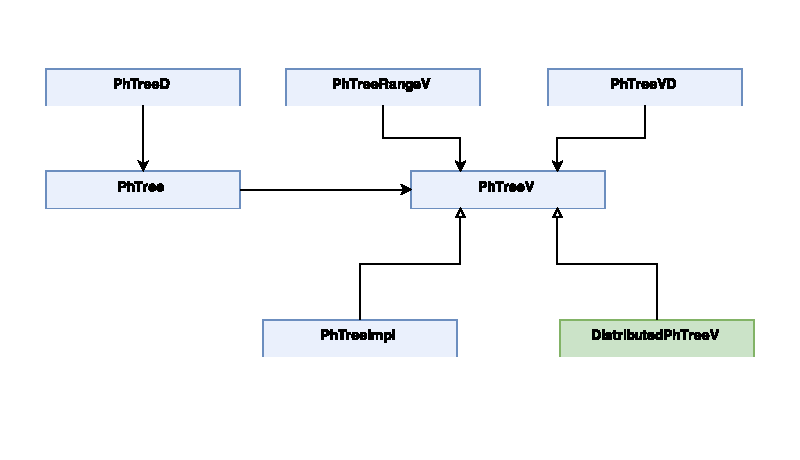
\includegraphics[scale=1]{images/PH-Tree-API}
    \caption{The Java API of the PH-tree. The classes coloured with blue represent the existing code, the additions in green represent the distributed implementation.}
    \label{fig:PH-tree-Java-API}
\end{figure}

The initial PH-tree implementation also provides support for range tree, which can store \textit{hyper-rectangles} defined by two multi-dimensional points: the bottom-left and top-right corners of the hyper-rectangle. These types of trees are implemented using special types of pre and post processors and are internally backed by point PH-trees. \textit{PhTreeRangeV} stores hyper-rectangles defined by multi-dimensional points represented as \textit{long[]} and allows arbitrary values. \textit{PhTreeRangeVD} is similar but allows points to be represented as \textit{double[]}. Both of these two implementations use an instance of \textit{PhTreeV} to store the processed hyper-rectangles, as shown in Figure \ref{fig:PH-tree-Java-API}. Finally, \textit{PhTreeRangeD} provides support for hype-rectangle set index is backed by a \textit{PhTree} object. 

As presented in Figure \ref{fig:PH-tree-Java-API}, all of the types of trees discussed depende on the interface PhTreeV. The distributed PH-tree provides another implementation for this interface. Method calls to any of the trees in the presented hierarchy are transformed into commands send by the \textit{DistrbutedPhTreeV} class to the indexing hosts over the network. After the requests are services, \textit{DistributedPhTreeV} combines the responses and provides the appropriate returning value. 

One big advantage of this approach is that client is not aware if it is using a in-memory tree or a distributed one, except at the creation time. Therefore, appliation previously using the in-memory version of the PH-tree can easily switch to the distributed implementation, with minimal code changes. 

The choice of providing a separate implementation only of the \textit{PhTreeV} class has another important consequence: the indexing hosts only need to maintain an in-memory instance of a \textit{PhTreeV} implementation, independent of the type of tree used by the client. This simplifies the implementation and also has the advantage of off-loading the pre and post processing operation from the servers to the clients, allowing faster request processing and better throughput on the servers. 
\section{Distribution}

\subsection{Client design}

A high level diagram of the client library is presented in Figure \ref{fig:Client-library}. The \textit{DistributedPhTreeV} class implements the \textit{PhTreeV} interface and provides access the distributed PH-tree. Each method call on the \textit{PhTreeV} interface is delegated to a \textit{PhTreeIndexProxy} object. This object converts each method call into a \textit{Request} object, similar to the \textit{Command design pattern}\footnote{http://en.wikipedia.org/wiki/Command\_pattern}. The proxy class also decides which hosts need to be contacted to resolve the operation, based on a locally cached \textit{Key-Mapping} object. This object contains the most recent cluster configuration available to the host. The \textit{Request} object is then passed on to a \textit{RequestDispatcher}, where it is encoded to an array of bytes and sent to the corresponding hosts via TCP sockets. The \textit{Transport} class keeps the most recently used connections alive, to avoid having to perform the TCP handshake for each operation when repeatedly interacting with the same host. 

\begin{figure}[h]
    \centering 
    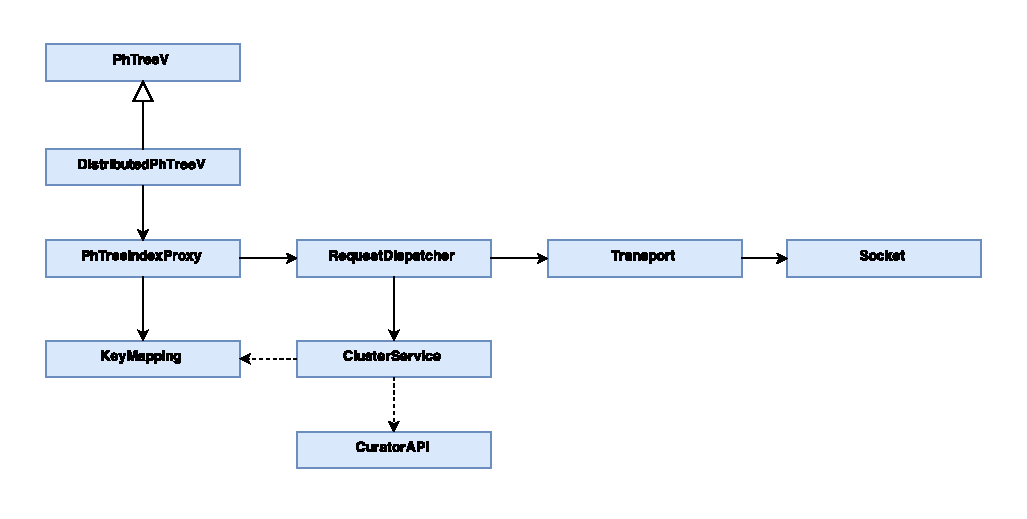
\includegraphics[scale=1]{images/Client}
    \caption{The class diagram of the client library}
    \label{fig:Client-library}
\end{figure}

The calls to the \textit{DistributedPhTreeV} methods are blocking, as the \textit{Transport} object blocks the execution until it has received a response from the remote indexing host. The response is received as an array of bytes and is decoded into a \textit{Response} object and returned to the \textit{RequestDispatcher} object. If more hosts participated in the query, their corresponding \textit{Response} objects are combined and the result of the operation is returned to the caller of the \textit{DistributedPhTreeV} method. 

\subsection{Server design}

The \textit{server library} is implemented as a multi-threaded, asynchronous, event-driven server, according to the \textit{reactor pattern}\footnote{http://en.wikipedia.org/wiki/Reactor\_pattern}. This model uses two types of threads: \textit{Dispatcher} threads and \textit{Handler} threads. A \textit{Dispatcher} thread accepts incoming connections, allocates the necessary resources to the connections and then passes the connection resources to a \textit{Handler} thread. The \textit{Handler} thread accepts requests from the client using the connection resource provided by the \textit{Dispatcher} thread. For the TCP protocol, this resource is generally and reference to a \textit{Socket} object. The \textit{Handler} thread manages requests from more than one client by leveraging the event-based IO support provided by the operating systm. The \textit{Netty IO} Java library was used for the implementation, as it provides an easy manner to set up the a pool of \textit{Handler} threads. The chosen server architecture generally performs better than architecturs which create a new thread for every request, as the \textit{Handler} threads are pooled and are initialized before any client requests are serviced. 

The high level diagram of the server library is presented in Figure \ref{fig:Server-library}. The main class of the \textit{server library} is the \textit{IndexMiddleware} class, which sets up the pool of handler threads and starts the dispatcher thread. The \textit{MiddlewareChannelHandler} class is the first handler that is executed by one of the \textit{Handler} threads upon receiving a request on a client connection. This class performs reads all of the bytes corresponding to a single request from a client and places them into a byte array object. This object is then passed to an instance of the \textit{IOHandler} class, which coverts the byte array into a \textit{Request} object. The \textit{IOHandler} then passed the \textit{Request} object to another handle, based on the type of the request. Client requests are passed along to a \textit{RequestHandler} object, while balancing requests, coming from othr servers are passed to the \textit{BalancingRequestHandler} object. 

\begin{figure}[h]
    \centering 
    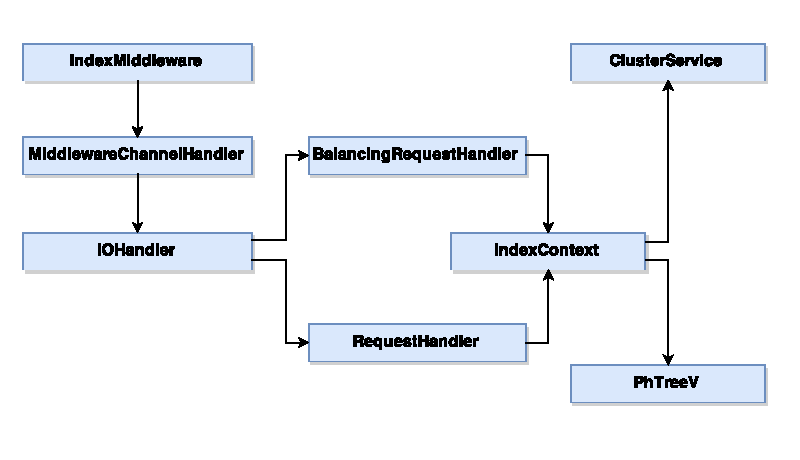
\includegraphics[scale=1]{images/Server}
    \caption{The class diagram of the server library}
    \label{fig:Server-library}
\end{figure}

Information that is commonly accessed by all of the \textit{Handler} threads is stored in the \textit{IndexContext} object. This object contains a reference to the \textit{ClusterService}, used to read and writer cluster configuration data, and to the in-memory PH-tree instance on that server, which is used in processing the client requests. 

\subsection{Configuration server and Key-Mapping implementation}

The \textit{Key-Mapping} was implemented using the ZooKeeper, an open-source coordination service. ZooKeeper provides access to a shared hierarchical namespace similar to a file system. This namespace is comprised of data registers, called \textit{znodes}, which are identified by a path and store data in the form of a byte array. The data stored within a \textit{znode} is guaranteed to always be read and written atomically. Additionally, each \textit{znode} can have any number of children \textit{znodes}. ZooKeeper provides primitives to create and delete \textit{znodes}, check if a node exists, get and set the data stored by a node and also retrieves the list of children of a node. It is also possible to set \textit{watches} on certain znodes, and receive notifications from ZooKeeper when the data of the node was changed. 

Both the client and the servers access the configuration data using the \textit{ClusterService} object, which maintains a cached version of the configuration on a \textit{KeyMapping} object. Handlers in the \textit{server library} module can also update the configuration through the \textit{ClusterService} API. The \textit{ClusterService} receives notifications from the ZooKeeper server when any data was changed updates the \textit{Key-Mapping} object with these updates. The implementation of the \textit{ClusterService} uses the \textit{Curator}\footnote{http://curator.apache.org/} framework, a set of libraries that provide a simpler and more reliable API for accessing ZooKeeper. 

\begin{figure}[h]
    \centering 
    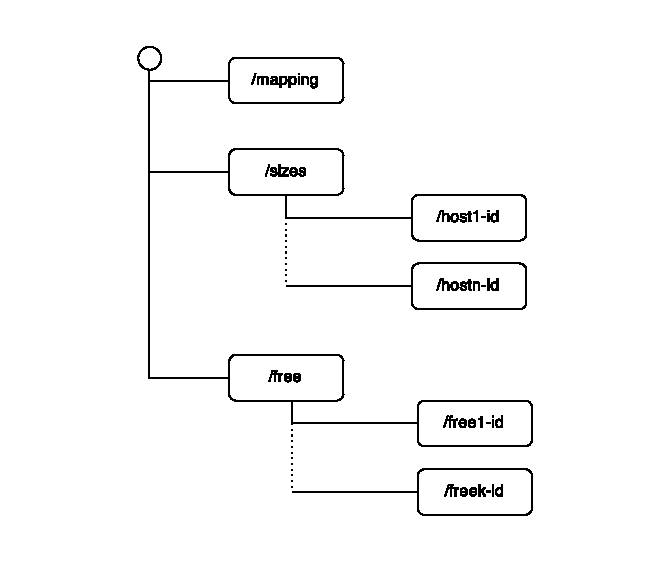
\includegraphics[scale=1]{images/KeyMapping}
    \caption{A diagram of the Key-Mapping stored in ZooKeeper}
    \label{fig:KeyMapping}
\end{figure}

The ZooKeeper configuration for the distributed PH-tree was implemented using three main znodes:
\begin{itemize}
    \item The \textit{/mapping} \textit{znode} contains the set of all Z-order intervals, together the host responsible for each of these intervals. All of this information is serialized into a byte array and is always read and written atomically by the indexing hosts. This is done to ensure that all Z-order intervals are read by the clients in an atomic manner, and always offer them a consistent view of the system. 
    \item The \textit{/sizes} znode stores an approximation of the number of entries stored in each indexing host, which is needed to make decisions during the \textit{re-balancing} operation. This znode contains one child znode for each host, the child node storing the approximate size of each host. This allows all of the hosts to update their size without clashing with updates from other hosts. Even though this means that the sizes of all of the hosts cannot be read atomically, the consistency loss is not significant, as the balancing operations do not require the precise number of entries stored on the neighbours. 
    \item Finally, the \textit{/free} znode contains a list of hosts which have registered themselves as free on start-up and will be contacted by the balancing initiators during the next balancing operations.
\end{itemize}

As the client maintain a cached copy of the latest information in ZooKeeper, it is possible that, due to network delays, the mapping on the client be different from the actual intervals on the server. Consider the following situation: a client initiates a query and after analyzing the local \textit{Key-Mapping}, it decides it has to contact host $h$ to retrieve the value for a certain key $k$. However, before the request reaches host $h$, this host could have already participated in a re-balancing operation and moved a part of its entries to a neighbouring host. If the entry involved in the query was moved to a different host, host $h$ no longer has it and would respond to the client that no such host exists in the cluster. This is wrong, as the entry was simply moved to a neighbouring host. To prevent this type of situations, the \textit{Key-Mapping} has a version number that is incremented after each re-balancing operation. Each indexing host stored the version of the mapping that was generated during the last re-balancing operation in which that host was involved. Furthermore, the clients include the version number of their local mapping in the requests sent to the hosts. Upon receiving a request, the server checks the client mapping version against the version of its last re-balancing operation. If the client version number is higher or equal, the request can be serviced without any consistency loss, as any changes that may have increase the clients version happened to other intervals in the mapping. Instead, if the client's version number is smaller than the host's version, the client is noticed that it's mapping is outdated and should retry the query. The client keeps attempting to send queries to indexing servers until it has received a response for an up to date mapping. 

In a cluster of $n$ hosts, there can be at most $n/2$ balancing operations running in parallel on the cluster. Therefore, it is important that a host's updates to the mapping do not overwrite the changes made by other hosts. The mapping update operation is performed in a \textit{compare-and-swap} manner, using the multi-update operation support provided by ZooKeeper. Using this type of operation, it is possible to perform an update to a znode only if its version (or alternatively, another znode's version) has not changed since the previous value was read. Following a re-balancing operation, the initiator hosts attempt to write the new version of the mapping to ZooKeeper. If the mapping was changed by another host, the initiator reads the new mapping, applies its changes on the interval bounds and retries the operation until it is successful. While this approach can lead to starvation if host is consistently blocked by other hosts to update the mapping, the situation is not likely to happen. An alternative solution to this problem would have been to implement a distributed lock on the mapping through ZooKeeper. In that situation, the initiators would always need to perform three requests to ZooKeeper: one request to acquire the lock, the second to perform the write and the third to release the lock. Our solution optimizes the duration of the re-balancing operation for the best case, when the write will be successful, as that situation is much more common in practice. 

\subsection{Communication protocol}

The distributed PH-tree uses a custom binary protocol for both the communication between a client and an indexing host and between two indexing neighbouring indexing hosts. The main communication flow is described in Figure \ref{fig:Encoding}. The \textit{RequestDispatcher} on the client creates a \textit{Request} object for each method call to the PH-tree API. This request object contains the request type and the arguments received by the method and it is converted into an array of bytes by the \textit{RequestEncoder} class, according to the communication protocol. The array of bytes is sent through the network to all of the servers that participate in the operation. On the server, the request is assigned to one of request processing threads which converts the array of bytes back to a \textit{Request} object using a \textit{RequestDecoder}. The request is then serviced by a \textit{RequestHandler} object, which returns a \textit{Response} object containing the result of the request. The \textit{Response} object is converted into an array of bytes using a \textit{ResponseEncoder} and sent back to the client over the wire. Back on the client, the response is decoded from a byte array. In case multiple servers were contacted, all of their responses are decoded and then combined to produce the return value of the method call.

\begin{figure}[h]
    \centering 
    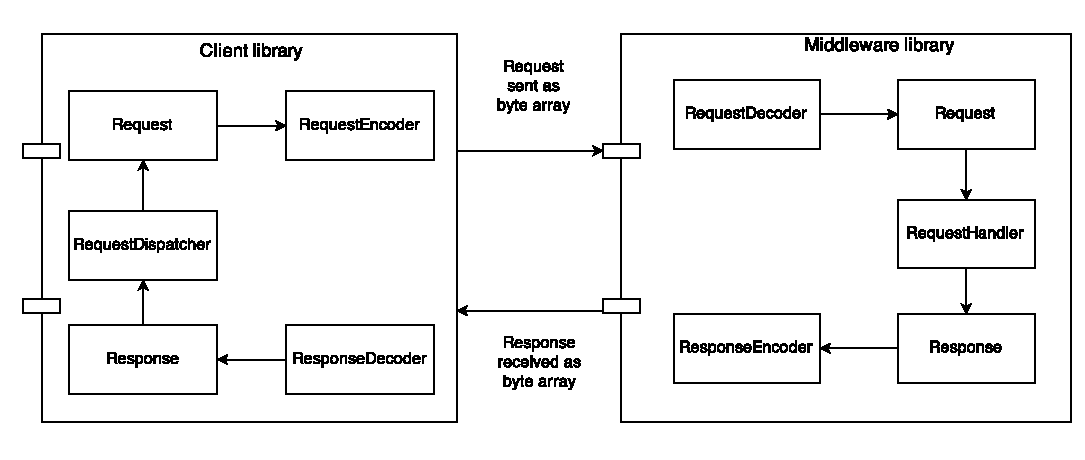
\includegraphics[scale=0.7]{images/Encoding}
    \caption{A diagram of the communication protocol between the client and the server}
    \label{fig:Encoding}
\end{figure}

The main reasons for using a binary protocol, as opposed to a more high level protocol based on JSON\footnote{http://json.org/} or XML\footnote{http://en.wikipedia.org/wiki/XML} are the following:
\begin{itemize}
    \item A binary protocol produces a much smaller output than a text based protocol. In the case of the custom binary protocol, all parameters are converted into arrays of bytes of the smallest possible size and combined into a large byte array. JSON and XML formats require additional metadata to store the name of the fields and to make the representation human readable. 
    \item JSON or XML protocols follow a two-step process: first the request is converted into a JSON or XML document, then the document is converted into an array of bytes to be sent over the network. The binary protocol skips the middle step and transforms requests directly into arrays of bytes. This makes the binary encoding faster than the text-based alternatives.
    \item The messages exchanged for this communication protocols are generally quite simple and thus the implementation effort for efficient custom serialization is not very high. 
\end{itemize}

\subsection{Iterators}

Beside the number of queries that return a list of entries that match certain parameters, the PH-tree API also provides support for iterators. These iterators implement the Java iterator API and allow clients to iterator over all of the entries of the tree or over all of the entries that fall within a certain query hyper-rectangle.

Once an iterator is created using the client API, the client sends a request to the host holding the first key in the iterator. This host creates an in-memory iterator object that is maintained until the client has finished iterating over the entries. The client retrieves batches of entries from the iterator on the host, to avoid having to send a request each time the iterator is moved a single position. Once all entries in the iterator stored on a single host have been exhausted, the client contacts the host holding the following portion of the iterator data and repeats the procedure. One advantage of this approach is that the client does not have to perform a network request for each entry of the iterator. Secondly, for iterators over large areas, spanning multiple hosts, it might also be unfeasible to request all of the entries in the iterator from all of the hosts and just iterator over them in-memory, on the client machine. A potential drawback of this solution is that each iterator running on a client has an associated iterator object running on an server machine. Thus, creating very large numbers of iterators could lead to large memory consumption on the servers and could potentially affect the performance in a negative manner.

\section{Concurrency}

The addition of concurrent support to the PH-tree involves the modification of the write operations to handle accesses from multiple threads. The operations which perform queries, create or execute iterators across the PH-tree were not modified, to preserve the response time of the read operations. Therefore, only the \textit{put()}, \textit{delete()} and \textit{updateKey()} methods for implementations of the \textit{PhTreeV} interface require modifications to support concurrency. 

The implementation was performed by isolating the write methods into a separate interface called \textit{PhOperations}. Thus, the PH-tree implementation delegates the execution of the write methods to an internal \textit{PhOperations} object. This pattern allows us to easily provide multiple implementation for concurrent write access strategies by placing each strategy into a separate implementation class. 

\begin{figure}[h]
    \centering 
    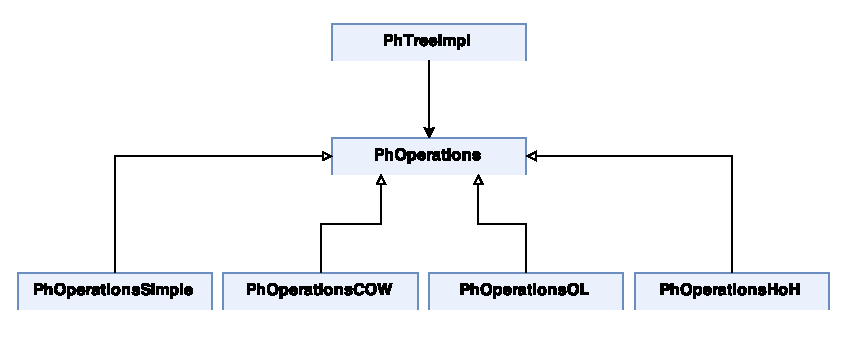
\includegraphics[scale=1]{images/PH-tree-concurrency}
    \caption{The Java API of the concurrency classes}
    \label{fig:Concurrency-classes}
\end{figure}

Figure \ref{fig:Concurrency-classes} shows the \textit{PhOperations} interface and its implementations. First of all, \textit{PhOperationsSimple} provides an no-concurrency implementation of the write operations, allowing operation that do not require concurrent access to by-pass the response time performance penalty added by the synchronized implementations. \textit{PhOperationsCOW} provides a full Copy-on-Write implementation, which essentially creates a "new" version\footnote{Only a single path from the root to the update node is changed at each write operations, the rest of the tree is shared with the previous version.} of the tree at each write operation and supports iteration on snapshots of the tree. This implementation supports a single writing accessing the three concurrently with an arbitrarily large number of readers. \textit{PhOperationHoH} and \textit{PhOperationsOL} are fine grained lock-based concurrency strategies, providing support for multiple reader and writer threads at the cost of strict consistency. In both of these implementations, the nodes modified are first copied and the modified copies are atomically replaced in the parent nodes. This removes the need for taking locks in the read methods. \textit{PhOperationsHoH} implements the tree descent using hand-over-hand locking, while \textit{PhOperationsOL} performs optimistic locking for this purpose. As previously discussed in Chapter \ref{ch:concurrency}, \textit{PhOperationsOL} may need multiple descents on the tree until the locking attempt was successful and should generally perform better than \textit{PhOperaionsHoH} for workloads in which the writers are not accessing the same area of the tree at the same time.

Another big advantage is that the \textit{PhOperations} reference can be swapped at runtime, which changes the concurrency strategy used by the PH-tree. This allows a tree to use optimistic locking while it is "loaded" with entries from multiple threads, and then switch to copy-on-write to allow iterators or range queries to execute on snapshots of the tree. 

\chapter{Evaluation}
\label{ch:evaluation}

\textit{Meta - will be removed after editing.}
\textit{Explain how the system should be evaluated, present and explain the benchmarks}

\chapter{Conclusions}
\label{ch:conclusions}

\section{Contributions}
\label{sec:conclusions-contribution}

This work presents a complete solution from implementing a distributed and parallel multi-dimensional index, by presenting both a distribution architecture and operation parallelization solutions for individual machines. The main contributions are the following:

The distribution architecture partitions the multi-dimensional space in a manner that allows fast point operation and efficient range and nearest neighbour queries. The proposed balancing algorithm ensures that all hosts will eventually hold a comparable number of entries, even in the case of very skewed input distributions. The presented distribution solution can be easily adapted for other types of index keys, as long as the key domain can be mapped to 1 dimensional line, allowing the constructing of efficient and scalable range-queryable, distributed key-values stores.

The in-memory PH-tree was updated to support concurrent access according to two consistency paradigms. The Copy-On-Write approach offers full consistency guarantees, providing snapshot semantics to queries and isolating readers from any further modifications to the tree. For situations where full consistency is not needed, the optimistic locking approach offers relaxed consistency semantics and provides improved write throughput by allowing concurrent write operations. Furthermore, none of presented approaches require the readers to acquire any locks and thus add no overhead to the execution of the read operations. 
\section{Future work}
\label{sec:conclusions-future-work}

One aspect of the distributed PH-tree that could be improved is the execution of the distributed nearest neighbour queries. As previously mentioned in section \ref{sec:distindex-algorithms}, the nearest neighbour algorithm first obtains the k nearest neighbours from the host responsible for the query point and then procees to run a range query on the cluster to check for any closer points on different hosts. The additional check is done by checking a hyper-cubic section of the initial space. A more efficient approach would be to check a hyper-spheric region centered in the query point. This improvement could reduce the number of hosts queried on the second step of the nearest neighbour queries and could potentially improve the execution time of such queries. 

From the point of view of the balancing algorithm, hosts participating in re-balancing operation do not accept write requests, to simplify the management of the mapping between the points and the hosts. The balancing algorithm could be modified to allow the hosts to accept write requests to a separate buffer and integrate the buffer to the stored PH-tree after the balancing operation has finished.

The concurrency strategies presented by this work rely on locking and copy-on-write to allow concurrent access. Further work could focus on investigating potential concurrent access strategies using on atomic operations.
\appendix

\listoffigures
\listoftables

\chapter*{Acknowledgements}

\newpage
\thispagestyle{empty}

\bibliographystyle{plain}
\bibliography{bibliography}

\end{document} 
